\chapter{反三角函数与简单三角方程的解法}
\section{反正弦函数}
我们知道,正弦函数$y=\sin x$是一个周期等于$2\pi$的振动函
数,它的定义域是$(-\infty,+\infty)$, 而值域是闭区间$[-1,1]$, 它的图象如图9.1。

\begin{figure}[htp]
    \centering
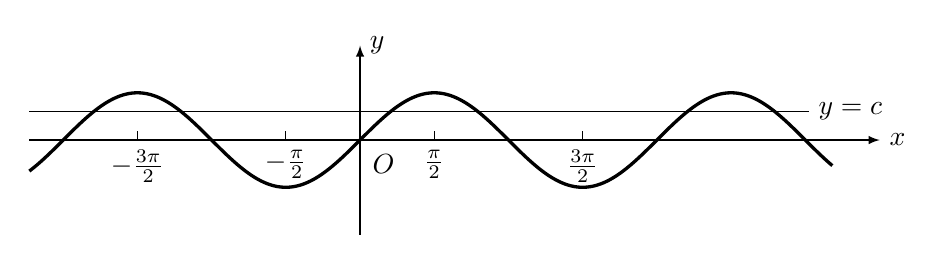
\begin{tikzpicture}[>=latex, scale=.6]
\draw[->] (-7,0)--(11,0)node[right]{$x$};
\draw [->] (0,-2)--(0,2)node[right]{$y$};

\draw[domain=-7:10, samples=1000, very thick] plot(\x,{sin(\x r)});
\draw  (-7,.6)--(9.5,0.6)node[right]{$y=c$};

\foreach \x/\xtext in {-1.5*pi/-\frac{3\pi}{2}, -.5*pi/-\frac{\pi}{2},.5*pi/\frac{\pi}{2}, 1.5*pi/\frac{3\pi}{2}}
{
    \draw (\x,0)node[below]{$\xtext$}--(\x,.2);
}
\node at (.5,-.5){$O$};
\end{tikzpicture}
    \caption{}
\end{figure}


每取一数$y=c,\; -1\le c\le 1$, 作直线$y=c$, 可与正弦曲线
$y=\sin x$交于无穷多个点,这些交点的横坐标是
\[x=x_0+2k\pi\qquad \text{和}\qquad x=(\pi -x_0)+2k\pi\quad (k\in\mathbb{Z})\]
因此有无数多个$x$的值满足方程$\sin x =c$, 而和那个$y=c$对
应。可见对于变数$x$的一切可能实数值来说,我们不能由函
数$f:\mathbb{R}\to [-1,1]$, $f(x)=\sin x$得出它的反函数来。把定
义域分成无数个单调区间,则在各区间$\left[-\frac{\pi}{2}+2k\pi, \frac{\pi}{2}+2k\pi\right]$上,$y=\sin x$由$-1$上升到1,而在各区间$\left[\frac{\pi}{2}+2k\pi, \frac{3\pi}{2}+2k\pi\right]$上,$y=\sin x$由1下降到$-1$,于是由前一章中的
反函数定理知道,对于上述每一个单调区间存在一个反函数。

如果我们强调的是在闭区间$\left[-\frac{\pi}{2},\frac{\pi}{2}\right]$上
来考虑正弦
函数的反函数,我们就说它是反正弦函数的主值,并把这个函数记作
$x=\arcsin y$,使得
$$x=\arcsin y\qquad \Longleftrightarrow \qquad y=\sin x$$
这里$x\in \left[-\frac{\pi}{2},\frac{\pi}{2}\right],\quad y\in[-1,+1]$。

对于使得$y=\sin x$是单调的另一区间,例如$x\in \left[\frac{\pi}{2},\frac{3\pi}{2}\right]$,
我们就得到另一个反正弦函数。假如我们没有明确地
指出反正弦函数的值域所在的区间,我们就不能由函数$y=\sin x$得出它的反函数。为了明确起见,现在我们规定

\begin{blk}{定义1}
    函数$y=\sin x$在闭区间$\left[-\frac{\pi}{2},\frac{\pi}{2}\right]$上
的反函数
叫做\textbf{反正弦函数}或\textbf{反正弦},这个函数用记号写作
$x=\arcsin y$ (即$x$是一角或弧,其相应的正弦值为$y$),
它的定义域是闭区间$-1\le y\le 1$, 值域是闭区间$-\frac{\pi}{2}\le x\le \frac{\pi}{2}$。
\end{blk}

用习惯上的写法,将字母$x$与$y$互换而写成$y=\arcsin x$,
现在,我们将反正弦函数(主值)的定义用几何名词叙述
如下:

在闭区间$-1\le x\le 1$上,数$x$的反正弦$y=\arcsin x$是在
闭区间$\left[-\frac{\pi}{2},\frac{\pi}{2}\right]$上
的一个角或弧,它的正弦值等于$x$, 
即$\sin y=x$.

由反正弦函数的定义和前一章的反函数定理可得到
它的一些性质如下:
\begin{itemize}
    \item $\arcsin(\sin y)=y,\qquad -\frac{\pi}{2}\le y\le \frac{\pi}{2}$
    
    $\sin(\arcsin x)=x,\qquad -1\le x\le 1$

    \item 函数$f(x)=\arcsin x$在闭区间$[-1,1]$上单调递
    增,并且连续。
    \item $y=\arcsin x,\; -1\le x\le 1$的图象与$y=\sin x,\; -\frac{\pi}{2}\le y\le \frac{\pi}{2}$
    的图象关于直线$y=x$对称(图5.2)。
\end{itemize}

\begin{figure}[htp]
    \centering
\begin{tikzpicture}[>=latex, scale=1]
\draw[->] (-4,0)--(4,0)node[right]{$x$};
\draw [->] (0,-3)--(0,3)node[right]{$y$};

\draw[domain=-pi:pi, samples=1000, dashed, thick] plot(\x,{sin(\x r)});
\draw[domain=-1:1, samples=1000, very thick] plot(\x,{asin(\x)*pi/180});
\draw[dashed] (-3,-3)--(2.5,2.5)node [above]{$y=x$};
\draw [dashed] (0,.5*pi)node[left]{$\frac{\pi}{2}$}--(1,.5*pi)node[above]{$y=\arcsin x$};
\draw [dashed] (0,-.5*pi)node[right]{$-\frac{\pi}{2}$}--(-1,-.5*pi);
\node at (.25,-.25){$O$};
\node at (pi+.5,0)[above]{$y=\sin x$};
\foreach \x in {-1,1}
{
    \draw (\x,0)node[below]{$\x$}--(\x,.1);
}
\draw (0,1)node[left]{$1$}--(.1,1);
\draw (0,-1)--(-.1,-1)node[right]{$-1$};

\end{tikzpicture}
    \caption{}
\end{figure}



我们已知正弦函数是奇函数,它的图象关于原点对称,
现在我们要证明 $f(x)=\arcsin x$是奇函数,即
$\arcsin(-x)=-\arcsin x$。

\begin{proof}
    因为$-\frac{\pi}{2}\le \arcsin x\le \frac{\pi}{2}$,
    角$-\arcsin x$也被限制在由$-\frac{\pi}{2}$到$\frac{\pi}{2}$
    的区间内:
    $$-\frac{\pi}{2}\le -\arcsin x\le \frac{\pi}{2}$$
    又,角$-\arcsin x$的正弦等于$-x$
\[\sin(-\arcsin x)=-\sin(\arcsin x)=-x\]
因此:$\arcsin(-x)=-\arcsin x$。
\end{proof}

\begin{example}
    求下列各式的值(口答):
    \begin{enumerate}
        \item $\arcsin\frac{1}{2}$
        \item $\arcsin\left(-\frac{1}{2}\right)$
        \item $\arcsin 1$
    \end{enumerate}
\end{example}

\begin{solution}
\begin{enumerate}
    \item $\arcsin\frac{1}{2}=\frac{\pi}{6}$,因为$\sin\frac{\pi}{6}=\frac{1}{2}$,且$-\frac{\pi}{2}<\frac{\pi}{6}<\frac{\pi}{2}$

    \item $\arcsin\left(-\frac{1}{2}\right)=-\frac{\pi}{6}$,因为$\sin\left(-\frac{\pi}{6}\right)=-\frac{1}{2}$,且
    $-\frac{\pi}{2}<-\frac{\pi}{6}<\frac{\pi}{2}$
    \item $\arcsin 1=\frac{\pi}{2}$,因为$\sin\frac{\pi}{2}=1$,而且$\frac{\pi}{2}$不超出$\left[-\frac{\pi}{2},\frac{\pi}{2}\right]$的界限。
\end{enumerate}
\end{solution}

\begin{example}
    求下列各式的值:
\[\arcsin\left(-\frac{\sqrt{3}}{2}\right),\qquad \arcsin (-0.2672) \]
\end{example}

\begin{solution}
\begin{enumerate}
    \item $\arcsin\left(-\frac{\sqrt{3}}{2}\right)=-\arcsin\frac{\sqrt{3}}{2}=-\frac{\pi}{3}$
    \item $\arcsin(-0.2672)=-\arcsin0.2672=-15^{\circ}30'\approx -0.2705$
\end{enumerate}
    
\end{solution}



\begin{example}
    求下列各式的值:
\begin{multicols}{2}
\begin{enumerate}
    \item $\sin\left(\arcsin\frac{1}{3}\right)$
    \item $\tan\left(\arcsin\frac{\sqrt{2}}{2}\right)$
    \item $\cos\left(\arcsin\frac{3}{5}\right)$
    \item $\sin\left[2\arcsin\left(-\frac{3}{5}\right)\right]$
    \item $\arcsin\left(\sin\frac{7\pi}{6}\right)$
\end{enumerate}
\end{multicols}
\end{example}

\begin{solution}
\begin{enumerate}
    \item $\sin\left(\arcsin\frac{1}{3}\right)=\frac{1}{3}$
    \item $\tan\left(\arcsin\frac{\sqrt{2}}{2}\right)=\tan\frac{\pi}{4}=1$
    \item 设$\arcsin\frac{3}{5}=\alpha$,其中$-\frac{\pi}{2}\le\alpha\le\frac{\pi}{2}$,那么$\sin\alpha=\frac{3}{5}$。由于$-\frac{\pi}{2}\le\alpha\le\frac{\pi}{2}$,$\sin\alpha>0$,可以知道,$\alpha$是第一象限的角,所以
    $$\cos\left(\arcsin\frac{3}{5}\right)=\sqrt{1-\left(\frac{3}{5}\right)^2}=\frac{4}{5}$$
    \item 设$\arcsin\left(-\frac{3}{5}\right)=\alpha$,其中$-\frac{\pi}{2}\le\alpha\le\frac{\pi}{2}$,那么
    \[\sin\alpha =\sin\left[\arcsin\left(-\frac{3}{5}\right)\right]=-\frac{3}{5}\]
由于$-\frac{\pi}{2}\le\alpha\le\frac{\pi}{2}$和$\sin\alpha<0$,可以知道$\alpha$是第四象限的角,所以
\[\cos\alpha=\sqrt{1-\left(-\frac{3}{5}\right)^2}=\frac{4}{5}\]
即:
$\sin\left[2\arcsin\left(-\frac{3}{5}\right)\right]=\sin2\alpha=2\sin\alpha\cdot \cos\alpha=2\left(-\frac{3}{5}\right)\cdot\left(\frac{4}{5}\right)=-\frac{24}{25}$
    \item \[\begin{split}
\arcsin\left(\sin\frac{7\pi}{6}\right)&=\arcsin\left[\sin\left(\pi+\frac{\pi}{6}\right)\right]\\
&=\arcsin\left(-\sin\frac{\pi}{6}\right)\\
&=-\arcsin\left(\sin\frac{\pi}{6}\right)=-\frac{\pi}{6}        
    \end{split}\]
\end{enumerate}
\end{solution}

关于$y=\sin x$, 只要知道了它在闭区间$-\frac{\pi}{2}\le x\le \frac{\pi}{2}$上
的反函数$x=\arcsin y$, 我们便能求出$y=\sin x$在其它单调区间
上的反函数。

\begin{blk}{命题}
\begin{enumerate}
    \item $y=\sin x$在闭区间$\left[-\frac{\pi}{2}+2k\pi,\frac{\pi}{2}+2k\pi\right]$上,由$-1$上升到1,它们相应的反函数是
\[x=\arcsin y+2k\pi,\quad k\in\mathbb{Z}\]
因为
\[\sin x= \sin(\arcsin y+ 2k\pi) = \sin(\arcsin y) = y\]
而且
\[-\frac{\pi}{2}+2k\pi\le \arcsin y+2k\pi \le \frac{\pi}{2}+2k\pi
,\quad k\in\mathbb{Z}\]
    
\item $y=\sin x$在闭区间$\left[\frac{\pi}{2},\frac{3\pi}{2}\right]$上,由1下降到$-1$,
它的反函数是
\[x=\pi-\arcsin y\]
因为
\[\sin x=\sin(\pi- \arcsin y) = \sin(\arcsin y) = y\]
而且
\[\frac{\pi}{2}=\pi-\frac{\pi}{2} \le \pi-\arcsin y \le \pi+\frac{\pi}{2}=\frac{3\pi}{2}\]
我们也可以在单位圆上作图来说明2,如图9.3所示。

\item $y=\sin x$在闭区间$\left[\frac{\pi}{2}+2k\pi,\frac{3\pi}{2}+2k\pi\right]$上,由
1下降到$-1$, 相仿地证得它在相应区间上的反函数是
\[x=(\pi-\arcsin y)+2k\pi,\quad k\in\mathbb{Z} \]
\end{enumerate}
\end{blk}

\begin{figure}[htp]
    \centering
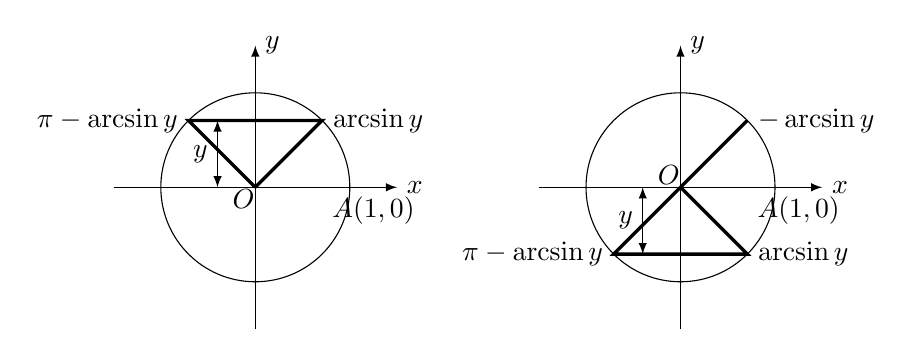
\begin{tikzpicture}[>=latex, scale=.6]
\begin{scope}
    \draw[->] (-3,0)--(3,0)node[right]{$x$};
    \draw[->] (0,-3)--(0,3)node[right]{$y$};
    \draw (0,0) circle(2);
    \node at (-.25,-.25){$O$};
\node at (2.5,0)[below]{$A(1,0)$};
\draw[very thick] (0,0)--(45:2)node[right]{$\arcsin y$}--(90+45:2)node[left]{$\pi-\arcsin y$}--(0,0);

\draw[<->] (-.8,0)--node[left]{$y$}(-.8,1.414);
\end{scope}

\begin{scope}[xshift=9cm]
    \draw[->] (-3,0)--(3,0)node[right]{$x$};
    \draw[->] (0,-3)--(0,3)node[right]{$y$};
    \draw (0,0) circle(2);
    \node at (-.25,.25){$O$};
\node at (2.5,0)[below]{$A(1,0)$};

\draw[<->] (-.8,0)--node[left]{$y$}(-.8,-1.414);
\draw[very thick] (0,0)--(-45:2)node[right]{$\arcsin y$}--(-90-45:2)node[left]{$\pi-\arcsin y$}--(0,0);
\draw[very thick] (0,0)--(45:2)node[right]{$-\arcsin y$};
\end{scope}
\end{tikzpicture}

    \caption{}
\end{figure}


\begin{example}
    讨论函数$y=\arcsin(\sin x)$的图象。
\end{example}

\begin{solution}
    由于正弦的周期性,函数$\arcsin(\sin x),\; x\in\mathbb{R}$也以
$2\pi$为周期,因此,只研究它在长度为$2\pi$的区间内情形即可。
由于
\[\sin y=\sin[\arcsin(\sin x)]=\sin x\]
这里$-\frac{\pi}{2}\le y\le \frac{\pi}{2}$,而$x\in\mathbb{R}$,故
\begin{itemize}
    \item 当$x\in\left[-\frac{\pi}{2},\frac{\pi}{2}\right]$时,则$y=x$。
    \item 当$x\in\left[\frac{\pi}{2},\frac{3\pi}{2}\right]$时,则由上面的命题2知
    \[x=\pi-y\quad \Rightarrow\quad y=\pi-x\in \left(-\frac{\pi}{2},\frac{\pi}{2}\right)\]
\end{itemize}
因之,在此区间内函数的图象与直线$y=\pi-x$一致,总之,
由上面的命题中的1和3的结果:
\begin{enumerate}
    \item 当$x\in \left[-\frac{\pi}{2}+2k\pi,\frac{\pi}{2}+2k\pi\right]$时,则$x=y+2k\pi$,则$y=x-2k\pi$;
    \item 当$x\in \left[\frac{\pi}{2}+2k\pi,\frac{3\pi}{2}+2k\pi\right]$时,则$x=\pi-y+2k\pi$,则$y=(\pi-x)-2k\pi$。
\end{enumerate}
由上面讨论的结果,得到函数$y= \arcsin
(\sin x)$的图象是折线的形状,如图5.4所示。
\begin{figure}[htp]
    \centering
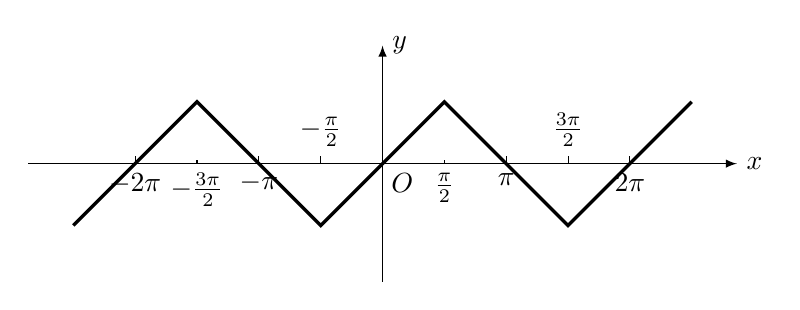
\begin{tikzpicture}[>=latex, scale=.5]
    \draw[->] (-9,0)--(9,0)node[right]{$x$};
    \draw[->] (0,-3)--(0,3)node[right]{$y$};
\draw[very thick] (-2.5*pi,-0.5*pi)--(-1.5*pi,.5*pi)--(-.5*pi,-0.5*pi)--(.5*pi,.5*pi)--(1.5*pi,-0.5*pi)--(2.5*pi,.5*pi);
\foreach \x/\xtext in {-2/-2\pi, -1/-\pi,1/\pi,2/2\pi}
{
    \draw (pi*\x,0)node[below]{$\xtext$}--(pi*\x,0.2);
}
\foreach \x/\xtext in {.5/\frac{\pi}{2},-1.5/-\frac{3\pi}{2}}
{
    \draw (pi*\x,0)node[below]{$\xtext$}--(pi*\x,0.1);
}
\foreach \x/\xtext in {1.5/\frac{3\pi}{2},-.5/-\frac{\pi}{2}}
{
    \draw (pi*\x,0)--(pi*\x,0.2)node[above]{$\xtext$};
}
\node at (.5,-.5){$O$};

\end{tikzpicture}
    \caption{}
\end{figure}
\end{solution}



\section*{习题9.1}
\addcontentsline{toc}{subsection}{习题9.1}
\begin{enumerate}
    \item 用反三角函数表示下面等式中的角。
    \begin{multicols}{2}
\begin{enumerate}
    \item $\sin\frac{\pi}{4}=\frac{\sqrt{2}}{2}$
    \item $\sin\frac{5\pi}{3}=-\frac{\sqrt{3}}{3}$
    \item $\sin\frac{7\pi}{3}=\frac{\sqrt{3}}{2}$
    \item $\sin(-2.314)=-0.04038$
\end{enumerate}
    \end{multicols}
    \item 当$\frac{1}{2}\le x\le\frac{\sqrt{3}}{2}$
    时,求函数$y=x\arcsin x$的最大值
    和最小值。
    \item 不求值,确定下面差的符号:
\begin{enumerate}
    \item $\arcsin 0.7-\arcsin 0.5$
    \item $\arcsin\left(-\frac{3}{5}\right)-\arcsin\left(-\frac{3}{4}\right)$
    \item $\arcsin\left(\sqrt{2}-1\right)-\arcsin\left(\sqrt{5}-2\right)$
\end{enumerate}
\item 求下列各式的值:
\begin{multicols}{2}
\begin{enumerate}
    \item $\arcsin\frac{\sqrt{3}}{2}$
    \item $\arcsin\left(-\frac{\sqrt{2}}{2}\right)$
    \item $\arcsin0$
    \item $\arcsin(-1)$
    \item $\arcsin\left(-\frac{1}{4}\right)$
    \item $\arcsin0.7841$
\end{enumerate}
\end{multicols}

\item 计算下列各式的值:
\begin{multicols}{2}
    \begin{enumerate}
        \item $\tan\left(\arcsin\frac{\sqrt{2}}{2}\right)$
        \item $\cos\left(\arcsin \frac{3}{5}\right)$
        \item $\arcsin \left[\sin\left(-\frac{\pi}{7}\right)\right]$
        \item $\arcsin\left(\sin\frac{5\pi}{6}\right)$
        \item $\arcsin(\cos1)$
    \end{enumerate}
    \end{multicols}
    \item 计算下列各式的值:
\begin{multicols}{2}
    \begin{enumerate}
        \item $\cot\left(2\arcsin\frac{\sqrt{2}}{2}\right)$
        \item $\cos\left(2\arcsin\frac{1}{3}\right)$
        \item $\sin\left(3\arcsin\left(-\frac{\sqrt{3}}{2}\right)\right)$
        \item $\tan\left(\frac{1}{2}\arcsin\frac{2}{3}\right)$
    \end{enumerate}
    \end{multicols}

    \item 讨论函数$y=x \arcsin(\sin x)$的图象,并作草图。
\item 画出$f(x)=\sin(3\arcsin x)$的图象。
\end{enumerate}

\section{反余弦函数}
由余弦函数$y=\cos x$的图象(图9.5)看出,函数$y=\cos x$
在闭区间$[2k\pi ,(2k+1)\pi ]$上,由1下降到$-1$, 而在闭区间
$[(2k-1)\pi ,2k\pi]$上,由$-1$上升到1; 因此,对于上述每一
个单调区间,函数$y=\cos x$都带来一个反函数。

\begin{figure}[htp]
    \centering
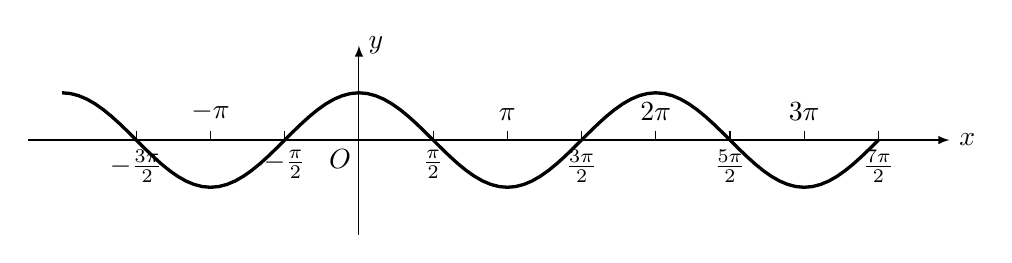
\begin{tikzpicture}[>=latex, scale=.6]
\draw[->] (-7,0)--(12.5,0)node[right]{$x$};
\draw[->] (0,-2)--(0,2)node[right]{$y$};
\foreach \x/\xtext in {-3/-\frac{3\pi}{2},-1/-\frac{\pi}{2},1/\frac{\pi}{2},3/\frac{3\pi}{2},5/\frac{5\pi}{2},7/\frac{7\pi}{2}}
{
    \draw(\x*pi/2, 0)node[below]{$\xtext$}--(\x*pi/2,.2);
}
\foreach \x/\xtext in {-1/-\pi, 1/\pi, 2/2\pi, 3/3\pi}
{
    \draw(\x*pi, 0)--(\x*pi,.2)node[above]{$\xtext$};
}
\draw [domain=-2*pi:3.5*pi, samples=100, very thick]plot(\x, {cos(\x r)});
\node at (-.4,-.4){$O$};
\end{tikzpicture}
    \caption{}
\end{figure}

\begin{blk}{定义2 }
    函数$y=\cos x$在闭区间$[0,\pi]$上的反函数叫做\textbf{反
余弦函数}或\textbf{反余弦},记作
\[x=\arccos y\]
它的定义域是闭区间$[-1,1]$。
\end{blk}

用几何名词来叙述这个定义,便是(互换字母$x$、$y$的
位置):在闭区间$-1\le x\le 1$上,数$x$的反余弦
$y=\arccos x$
是在闭区间$[0,\pi]$的一个角或弧,它的余弦值等于$x$, 即
$\cos y=x$。

\begin{example}
    求下列各式的值(口答):
    \begin{multicols}{2}
\begin{enumerate}
    \item $\arccos\frac{1}{2}$
    \item $\arccos\left(-\frac{1}{2}\right)$
    \item $\arccos1$
    \item $\arccos0$
\end{enumerate}
    \end{multicols}
\end{example}

\begin{solution}
\begin{enumerate}
    \item $\arccos\frac{1}{2}=\frac{\pi}{3}$,因为$\cos\frac{\pi}{3}=\frac{1}{2}$,而且$0<\frac{\pi}{3}<\pi$。
    \item $\arccos\left(-\frac{1}{2}\right)=\frac{2\pi}{3}$,因为$\cos\frac{2\pi}{3}=\cos\left(\pi-\frac{\pi}{3}\right)=\frac{1}{2}$,而且$0<\frac{2\pi}{3}<\pi$。
    \item $\arccos1=0$,因为$\cos 0=1$而且0不出$[0,\pi]$的界限。
    \item $\arccos0=\frac{\pi}{2}$,因为$\cos\frac{\pi}{2}=1$,而且$0<\frac{\pi}{2}<\pi$。
\end{enumerate}
\end{solution}

由反余弦函数的定义和反函数的定理得到反余弦的性质
如下:
\begin{enumerate}
\item $\arccos(\cos y)=y,\; 0\le y\le \pi,\qquad \cos(\arccos x)=x,\; -1\le x\le 1$
\item 函数$f(x)=\arccos x$在闭区间$[-1,1]$上,由$\pi$下
降到0, 且连续。
\item 我们知道互补的两个角$\alpha$和$\pi-\alpha$的余弦是相反
数,即
\[\cos(\pi-\alpha)=-\cos\alpha\]
反之,在区间$[-1,1]$内的相反数的反余弦互为补角,即
\[\arccos(-x)=\pi-\arccos x,\qquad x\in [-1,1]\]

\item 反余弦函数$y=\arccos x$的图象如图9.6所示。
\begin{figure}[htp]
    \centering
\begin{tikzpicture}[>=latex, scale=1.8]
    \draw[->] (-2,0)--(2,0)node[right]{$x$};
    \draw[->] (0,-.5)--(0,3.5)node[right]{$y$};
\draw[domain=-1:1, samples=1000, very thick] plot(\x, {acos(\x)*pi/180});
\node at (.1,-.1){$O$};
\foreach \x/\xtext in {-1/-1,1/1,-.4/-x,.4/x}
{
    \draw (\x,0)node[below]{$\xtext$}--(\x,.1);
}
\node at (0,.5*pi) [right]{$\frac{\pi}{2}$};
\node at (-1,pi) [left]{$y=\arccos x$};
\draw[dashed](-1,0)--(-1,pi)--(0,pi)node[right]{$\pi$};
\draw[dashed](-.4,0)--(-.4,1.98)--(0,1.98)node[right]{$\arccos(-x)$};
\draw[dashed](.4,0)--(.4,1.16)node[right]{$\arccos x$}--(0,1.16);

\end{tikzpicture}
    \caption{}
\end{figure}
\end{enumerate}

\begin{proof}
    因为$0\le \arccos(-x)\le \pi$, 又$0\le \pi -\arccos x\le x$
而且
\[\cos(\pi -\arccos x)=-\cos(\arccos x)=-x\]
由余弦函数在$[0,\pi]$ 上是单调的,得到
\[\pi -\arccos x=\arccos (-x)\]
\end{proof}

\begin{example}
    求下列各式的值:
$\arccos\left(-\frac{\sqrt{2}}{2}\right),\qquad \arccos(-0.9695)$
\end{example}


\begin{solution}
\[\arccos\left(-\frac{\sqrt{2}}{2}\right)=\pi-\arccos\left(\frac{\sqrt{2}}{2}\right)=\pi-\frac{\pi}{4}=\frac{3\pi}{4}\]
\[\begin{split}
    \arccos(-0.9695)&=180^{\circ}-\arccos0.9695\\
    &=180^{\circ}-14^{\circ}11'=165^{\circ}49'\approx 165.82^{\circ}\\
    &\approx 0.9212\pi\approx 2.894\text{弧度}
\end{split}\]
\end{solution}


\begin{example}
求$\tan\left[\arccos\left(-\frac{2\sqrt{2}}{3}\right)\right]$的值。
\end{example}

\begin{solution}
设$\arccos\left(-\frac{2\sqrt{2}}{3}\right)=\alpha$,其中$0\le \alpha\le \pi$,那么,$\cos\alpha=-\frac{2\sqrt{2}}{3}$,由于$0\le\alpha\le \pi$和$\cos\alpha<0$。可以知道$\alpha$是第二象限的角,所以
\[\tan\alpha=-\sqrt{\frac{1}{\cos^2\alpha}-1}=-\sqrt{\frac{9}{8}-1}=-\sqrt{\frac{1}{8}}=-\frac{\sqrt{2}}{4}\]
\end{solution}


\begin{example}
证明:若$|x|\le 1$,则$\arcsin x+\arccos x=\frac{\pi}{2}$

\end{example}

\begin{proof}
 $\because\quad    \sin\left(\frac{\pi}{2}-\arccos x\right)=\cos(\arccos x)=x$

    又    $\sin(\arcsin x)=x$, 且
  \[  0\le \arccos x\le \pi,\qquad -\frac{\pi}{2}\le \frac{\pi}{2}-\arccos x\le \frac{\pi}{2}\]

$\therefore\quad \arcsin x$和$\frac{\pi}{2}-\arccos x$是$\sin x$在单调区间$\left[-\frac{\pi}{2},\frac{\pi}{2}\right]$上的角。

根据$\sin x$在这区间上的单调性,有
$\arcsin x=\frac{\pi}{2}-\arccos x$
即:
\[\arcsin x+\arccos x=\frac{\pi}{2}\]
\end{proof}

\begin{example}
证明:$\arcsin\frac{4}{5}+\arccos\frac{12}{13}+\arcsin\frac{16}{65}=\frac{\pi}{2}$
\end{example}

\begin{proof}
\[\begin{split}
    \arcsin\frac{4}{5}+\arccos\frac{12}{13}&=\frac{\pi}{2}-\arcsin\frac{16}{65}\\
&=\arccos\frac{16}{65}
\end{split}\]
    
令$\alpha=\arcsin\frac{4}{5}$,则$\sin\alpha=\frac{4}{5}$,$0<\alpha<\frac{\pi}{2}$,$\cos\alpha=\frac{3}{5}$。

令$\beta=\arccos\frac{12}{13}$,则$\cos\beta=\frac{12}{13}$,$0<\beta<\frac{\pi}{2}$,$\sin\beta=\frac{5}{13}$。

因此:\[\begin{split}
    \cos(\alpha+\beta)&=\cos\alpha\cos\beta-\sin\alpha\sin\beta\\
    &=\frac{3}{5}\cdot \frac{12}{13}-\frac{4}{5}\cdot \frac{5}{13}=\frac{16}{65}
\end{split}\]

$\because\quad 0<\alpha+\beta<\pi$, $\therefore\quad \alpha+\beta=\arccos\frac{16}{65}$,即:
\[\arcsin\frac{4}{5}+\arccos\frac{12}{13}=\arccos\frac{16}{65}=\frac{\pi}{2}-\arcsin\frac{16}{65}\]

\[\therefore\quad \arcsin\frac{4}{5}+\arccos\frac{12}{13}+\arcsin\frac{16}{65}=\frac{\pi}{2}\]
\end{proof}

在余弦函数的其它单调区间内,其反函数可按下列方式
去找:

\begin{blk}{命题1}
\begin{enumerate}
    \item 在闭区间$[2k\pi ,(2k+1)\pi]$ 上,$y=\cos x$由
    1下降到$-1$, 在这些闭区间上的反函数是
 \[   x=\arccos y+2k\pi \]
    事实上,角$x\in [2k\pi ,(2k+1)\pi]$, 而且它的余弦等于$y$。
    \item 在闭区间$[(2k-1)\pi ,2k\pi]$ 上,$y=\cos x$的反函数
    是
\[    x=-\arccos y+2k\pi \]
    证明相仿。
\end{enumerate}
\end{blk}

\begin{example}
    讨论函数$y=\arccos(\cos x)$的图象。
\end{example}

\begin{solution}
因为$\cos x$的周期是$2\pi$, 函数$\arccos(\cos x)$也是周期函
数,周期是$2\pi$, 且
\[\cos y=\cos[\arccos(\cos x)]\]
即:
$\cos y=\cos x$, 这里$0\le y\le \pi$, $x\in\mathbb{R}$根据上面的命题,
知道:
\begin{enumerate}
    \item 当$x\in[2k\pi ,(2k+1)\pi]$ 时,$x=y+2k\pi$, 即
$y=x-2k\pi$;
\item  当$x\in[(2k-1)\pi ,2k\pi]$ 时,$x=-y+2k\pi$, 即
$y=-x+2k\pi$。
\end{enumerate}
函数$y=\arccos(\cos x)$的图象是折线(图5.7)。

\begin{figure}[htp]
    \centering
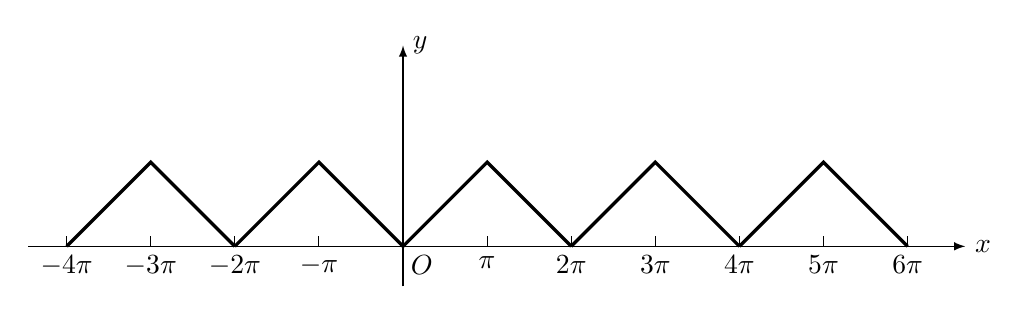
\begin{tikzpicture}[>=latex, scale=.34]
    \draw[->] (-14,0)--(21,0)node[right]{$x$};
    \draw[->] (0,-1.5)--(0,7.5)node[right]{$y$};
\foreach \x in {-4,-2,...,4}
{
    \draw[very thick] (\x*pi,0)--(\x*pi+pi,pi)--(\x*pi+pi+pi,0);
}
\foreach \x in {-4,-3,-2,2,3,4,5,6}
{
    \draw (\x*pi,0)node[below]{$\x\pi$}--(\x*pi,.4);
}
\foreach \x/\xtext in {-1/-\pi,1/\pi}
{
    \draw (\x*pi,0)node[below]{$\xtext $}--(\x*pi,.4);
}
\node at (.7,-.7){$O$};


\end{tikzpicture}    
    \caption{}
\end{figure}
\end{solution}


\section*{习题9.2}
\addcontentsline{toc}{subsection}{习题9.2}

\begin{enumerate}
    \item 用反余弦的形式表示下列各式的角($x\in[0,\pi]$)。
\begin{multicols}{2}
\begin{enumerate}
    \item $\cos\pi =1$
    \item $\cos\frac{5\pi}{3}=-\frac{1}{2}$
    \item $\cos(-3)=-0.9900$
    \item $\cos\frac{7\pi}{6}=-\frac{\sqrt{3}}{2}$
    \item $\cos x=-0.8065$
    \item $\cos x=-1$
\end{enumerate}
\end{multicols}

\item 决定下面差的符号:
\begin{multicols}{2}
\begin{enumerate}
 \item $\arccos0.7-\arccos0.5$
\item $\arccos\left(-\frac{3}{5}\right)-\arccos\left(-\frac{3}{4}\right)$
\item $\arccos\left(\sin\frac{\pi}{12}\right)-\arccos\left(\sin\frac{\pi}{13}\right)$
\end{enumerate}
\end{multicols}
\item 不作计算,确定下列各比的符号:
\begin{multicols}{2}
\begin{enumerate}
    \item $\frac{\arcsin0.85-\arcsin0.8}{\arccos0.85-\arccos0.8}$
    \item $\frac{\pi -2\arcsin(0.9)}{\pi -2\arccos(0.1)}$
    \item $\frac{\arcsin(0.4)+\frac{\pi}{6}}{\arcsin(0.6)-\frac{\pi}{3}}$
\end{enumerate}
\end{multicols}

\item 在同一个坐标系中,作函数$y=\arccos x$
和函数$y=\arccos\frac{x}{2}$
的图象,试根据函数图象说明当$x$为何值时,函数
的差$\arccos\frac{x}{2}-\arccos x$
取最大值、最小值、等于零。
\item 计算下列各式的值:
\begin{multicols}{2}
    \begin{enumerate}
\item $\sin \left(\arccos \frac{1}{2}\right)$
\item $\sin \left(\arccos \frac{3}{5}\right)$
\item $\tan \left(\arccos \frac{5}{13}\right)$
\item $\arcsin (\cos 1)$
\item $\arccos (\cos 2 \pi)$
\item $\arccos \left(-\cos \frac{36}{7} \pi\right)$
\item $\sin \left(\frac{1}{2} \arccos \frac{1}{2}\right)$
\item $\sin \left[3 \arccos \left(-\frac{\sqrt{3}}{2}\right)\right]$
\item $\sin \left[2 \arccos \left(-\frac{2 \sqrt{2}}{3}\right)\right]$
\item $\cos \left(\arcsin \frac{3}{5}-\arccos \frac{5}{13}\right)$    
\item $\sin\left[2\left(\arcsin\frac{\sqrt{5}}{3}-\arccos\frac{\sqrt{5}}{3}\right)\right]$
    \item $\tan\left(\arcsin\frac{1}{2}+\arccos\frac{\sqrt{3}}{2}\right)$
    \end{enumerate}
\end{multicols}

\item 证明下面的恒等式:
\begin{enumerate}
\item 若$0<x<1$, 则:
$\arcsin x=\arccos\sqrt{1-x^2}$
\item 若$0<x<1$, 则:
$\arccos x=\arcsin\sqrt{1-x^2}$
\item 若$-1\le x\le 0$, 则:
$\arcsin x=-\arccos\sqrt{1-x^2}$
\item 若$-1\le x\le 0$, 则:
$\arccos x=\pi-\arcsin\sqrt{1-x^2}$
\end{enumerate}

\item 解下面的方程:
    \begin{enumerate}
\item $\arccos x=\frac{\pi}{3}$
\item $\arccos 2x=0.5$
\item $\arcsin x=\arccos x,\; |x|\le 1$
\item $\arcsin x+\arcsin (1-x)=\arccos x$
\item $\arcsin x-\arccos x=\arcsin (3x-2)$
    \end{enumerate}

\item 当$-\frac{1}{2}\le x\le 0$时,求$f(x)
=\arccos x+x^2$的最小值。
\end{enumerate}

\section{反正切函数}

由正切函数$y=\tan x$的图象(图9.8)可以看出,函数$\tan x$
在每个开区间$\left(-\frac{\pi}{2}+2k\pi, \frac{\pi}{2}+2k\pi\right)$内,由$-\infty$上升到$+\infty$。
所以在每个这样的开区间里能带来一个反函数。


\begin{figure}[htp]
    \centering
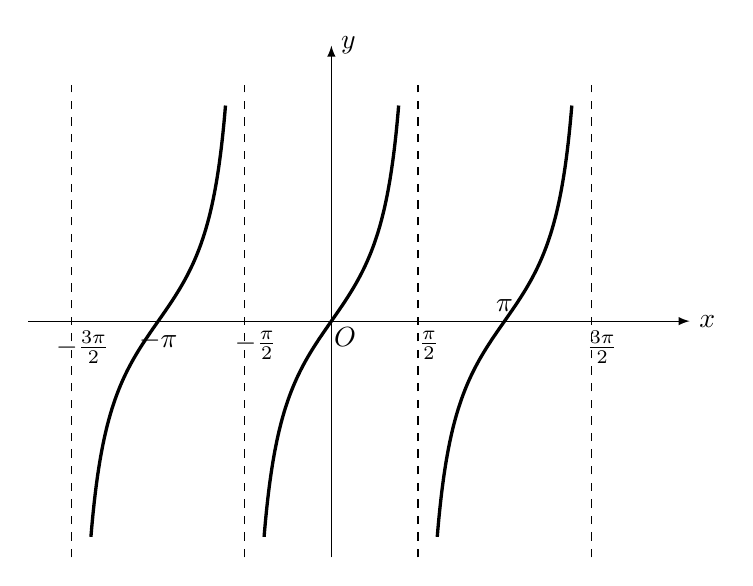
\begin{tikzpicture}[>=latex, xscale=.7]
    \draw[->] (-5.5,0)--(6.5,0)node[right]{$x$};
\draw[->] (0,-3)--(0,3.5)node[right]{$y$};
\foreach \x in {-.5,.5,1.5,-1.5}
{
    \draw[dashed] (\x*pi,-3)--(\x*pi,3);
}

\foreach \y in {-.5,.5,-1.5}
{
    \draw [domain=\y*pi+.35:(\y+1)*pi-.35, samples=1000, very thick] plot(\x, {tan(\x r)});
}

\node at (.25,-.2){$O$};
\node at (-pi,0)[below]{$-\pi$};
\node at (pi,0)[above]{$\pi$};

\node at (-.5*pi+.2,0)[below]{$-\frac{\pi}{2}$};
\node at (.5*pi+.2,0)[below]{$\frac{\pi}{2}$};
\node at (1.5*pi+.2,0)[below]{$\frac{3\pi}{2}$};
\node at (-1.5*pi+.2,0)[below]{$-\frac{3\pi}{2}$};
\end{tikzpicture}
    \caption{}

\end{figure}



\begin{blk}{定义3}
    函数$y=\tan x$在开区间$-\frac{\pi}{2}<x<\frac{\pi}{2}$
内的反函数叫做反正切函数 或 反正
切,记作
\[x=\arctan y\]
因为任何实数都可以作为正
切的值,所以反正切定义域是开区间$-\infty<y<+\infty$
\end{blk}

用几何名词来叙述反正
切的定义就是:在开区间
$(-\infty, +\infty)$内,数$y$的反
正切$x=\arctan y$是在开区间$-\frac{\pi}{2}<x<\frac{\pi}{2}$
内的一个角或弧,它的正切等于$y$,即:$\tan x=y$。

由定义和反函数定理直接得到反正切的性质如下:
\begin{enumerate}
    \item $\arctan (\tan x)=x, \qquad -\frac{\pi}{2}<x<\frac{\pi}{2}$
    
    $\tan (\arctan y)=y,\qquad -\infty<x<+\infty$
    \item $y=\arctan x,\; x\in\mathbb{R}$是单调递增的并且连续;
    \item $\arctan x$是奇函数,即
    \[\arctan (-x)=-\arctan x\]
    证明留给同学们去完成。
    \item 反正切函数$y=\arctan x,\; -\infty<x<+\infty$的图象如
    图5.9所示。
\end{enumerate}

\begin{figure}[htp]
    \centering
\begin{tikzpicture}[>=latex, scale=.7]
    \draw[->] (-5.5,0)--(6.5,0)node[right]{$x$};
    \draw[->] (0,-3)--(0,3)node[right]{$y$};
\draw[dashed] (-5.5,pi/2)--(6.5,pi/2);
\draw[dashed] (-5.5,-pi/2)--(6.5,-pi/2);

\draw [domain=-5.5:5.5, samples=100, very thick]plot(\x, {atan(\x)*pi/180});
\node at (.35,-.35){$O$};
\node at (0,2)[right]{$\frac{\pi}{2}$};
\node at (0,-2)[right]{$-\frac{\pi}{2}$};
\node at (5.5,pi/2-.3)[right]{$y=\arctan x$};
\end{tikzpicture}
    \caption{}
\end{figure}



\begin{example}
    求下列各式的值(口答):
\begin{multicols}{2}
\begin{enumerate}
    \item $\arctan 1$
    \item $\arctan (-1)$
    \item $\arctan \sqrt{3}$
    \item $\arctan (-\sqrt{3})$
\end{enumerate}
\end{multicols}
\end{example}

\begin{solution}
\begin{enumerate}
    \item $\arctan 1=\frac{\pi}{4}$,因为$\tan\frac{\pi}{4}=1$,而且$-\frac{\pi}{2}<\frac{\pi}{4}<\frac{\pi}{2}$
    \item $\arctan (-1)=-\frac{\pi}{4}$,因为$\tan\left(-\frac{\pi}{4}\right)=-1$,而且$-\frac{\pi}{2}<-\frac{\pi}{4}<\frac{\pi}{2}$
    \item $\arctan \sqrt{3}=\frac{\pi}{3}$,因为$\tan\frac{\pi}{3}=\sqrt{3}$,而且$-\frac{\pi}{2}<\frac{\pi}{3}<\frac{\pi}{2}$
    \item $\arctan (-\sqrt{3})=-\frac{\pi}{3}$,因为$\tan\left(-\frac{\pi}{3}\right)=-\sqrt{3}$,而且$-\frac{\pi}{2}<-\frac{\pi}{3}<\frac{\pi}{2}$
\end{enumerate}
\end{solution}

\begin{example}
    求$\cos\left[\arctan\left(-\frac{3}{4}\right)\right]$
\end{example}

\begin{solution}
设$\alpha=\arctan\left(-\frac{3}{4}\right)$,其中$-\frac{\pi}{2}<\alpha<\frac{\pi}{2}$,则$\tan\alpha=-\frac{3}{4}$。

由于$-\frac{\pi}{2}<\alpha<\frac{\pi}{2}$和$\tan\alpha<0$,可以知道$\alpha$是第四象限的角。所以
\[\begin{split}
    \sec\alpha&=\sqrt{1+\tan^2\alpha}=\sqrt{1+\frac{9}{16}}=\frac{5}{4}\\
    \cos\alpha&=\frac{4}{5}
\end{split}\]
就是
\[\cos\left[\arctan\left(-\frac{3}{4}\right)\right]=\cos\alpha=\frac{4}{5}\]
\end{solution}

关于$y=\tan x$在其它单调区间内的反函数,请看下面命题。

\begin{blk}{命题}
    在开区间$\left(-\frac{\pi}{2}+k\pi ,\frac{\pi}{2}+k\pi 
\right)$,$k\in\mathbb{Z}$内$y=\tan x$
由$-\infty$上升到$+\infty$, 在这些区间上的反函数是
$x=\arctan y+k\pi$。
\end{blk}

事实上,$x\in \left(-\frac{\pi}{2}+k\pi ,\frac{\pi}{2}+k\pi 
\right)$而
且
\[\tan x=\tan (\arctan y+k\pi )=\tan (\arctan y)=y\]




\begin{example}
    求$\arctan 2+\arctan 3$的值。
\end{example}

\begin{solution}
    $\because\quad \frac{\pi}{4}=\arctan 1<\arctan 2<\frac{\pi}{2}$,$\frac{\pi}{4}=\arctan 1<\arctan 3<\frac{\pi}{2}$,

    $\therefore\quad \frac{\pi}{2}<\arctan 2+\arctan 3<\pi$。而且
\[\begin{split}
    \tan(\arctan 2+\arctan 3)&=\frac{\tan (\arctan 2)+\tan (\arctan  3)}{1-\tan(\arctan 2)\cdot \tan (\arctan 3)}\\
    &=\frac{2+3}{1-2\x 3}=-1
\end{split}\]
由于$\arctan (-1)\in \left(-\frac{\pi}{2},0\right)$,于是
\[\arctan 2+\arctan 3=\arctan (-1)+\pi=-\frac{\pi}{4}+\pi=\frac{3\pi}{4}\]
\end{solution}

\begin{example}
    讨论 $y=\arctan (\tan x)$的图象。
\end{example}

\begin{solution}
函数$\arctan (\tan x)$的定义域是除去$x=\frac{\pi}{2}+k\pi,\; k\in\mathbb{Z}$
的实数集$\mathbb{R}$, 也就是无数个开区间$\left(-\frac{\pi}{2}+k\pi,\frac{\pi}{2}+k\pi\right),\; k\in\mathbb{Z}$
所组成的一个并集。因此函数$y=\arctan (\tan x)$的图象在
$x=\frac{\pi}{2}+k\pi,\; k\in\mathbb{Z}$这些点处间断。由于
\[\tan y=\tan[\arctan(\tan x)]\]
即:
$\tan y=\tan x$, 这里$-\frac{\pi}{2}<y<\frac{\pi}{2}$, $x\ne \frac{\pi}{2}+k\pi$。

所以,当$x\in\left(-\frac{\pi}{2}+k\pi,\frac{\pi}{2}+k\pi\right)$时,$x=y+k\pi$, 也就是$y=x-k\pi$。于是:
\begin{itemize}
    \item 当$x\in\left(-\frac{\pi}{2},\frac{\pi}{2}\right)$时,$y=x$;
    \item 当$x\in\left(\frac{\pi}{2},\frac{3\pi}{2}\right)$时,$y=x-\pi$;
    \item 当$x\in\left(\frac{3\pi}{2},\frac{5\pi}{2}\right)$时,$y=x-2\pi$;
    \item ………………
    \item 当$x\in\left(-\frac{3\pi}{2},-\frac{\pi}{2}\right)$时,$y=x+\pi$;
    \item ………………
\end{itemize}
现在考虑间断点的情形:

当$\frac{\pi}{2}+(k-)\pi<x<\frac{\pi}{2}+k\pi$时,$y=x-k\pi$, 于是当$x$
取每一个数列$\{x_n\}$从左边趋近$\frac{\pi}{2}+k\pi$ 时,记作
$x_n\to \left(\frac{\pi}{2}+k\pi \right)^-$, 
便有
\[\lim_{x_n\to \left(\tfrac{\pi}{2}+k\pi \right)^-}y=\lim_{x_n\to \left(\tfrac{\pi}{2}+k\pi \right)^-}(x_n-k\pi)=\frac{\pi}{2}+k\pi-k\pi=\frac{\pi}{2}\]

当$\frac{\pi}{2}+k\pi <x<\frac{\pi}{2}+(k+1)\pi$ 时,$y=x-(k+1)\pi$. 于
是当$x$取每一个数列$\{x_n\}$从右边趋近$\frac{\pi}{2}+k\pi$ 时,记作$x_n\to \left(\frac{\pi}{2}+k\pi\right)^+$,便有
\[\lim_{x_n\to \left(\tfrac{\pi}{2}+k\pi \right)^+}y=\lim_{x_n\to \left(\tfrac{\pi}{2}+k\pi \right)^+}[x_n-(k+1)\pi]=\frac{\pi}{2}+k\pi-k\pi-\pi=-\frac{\pi}{2}\]
因之,函数$\arctan(\tan x)$在间断点
$x=\frac{\pi}{2}+k\pi$处的左、右极
限存在,其左极限等于$\frac{\pi}{2}$
右极限等于$-\frac{\pi}{2}$,函数图象在
这些间断点处,有一个等于$\pi$ 的跃度,它的图象如图9.10。

\begin{figure}[htp]
    \centering
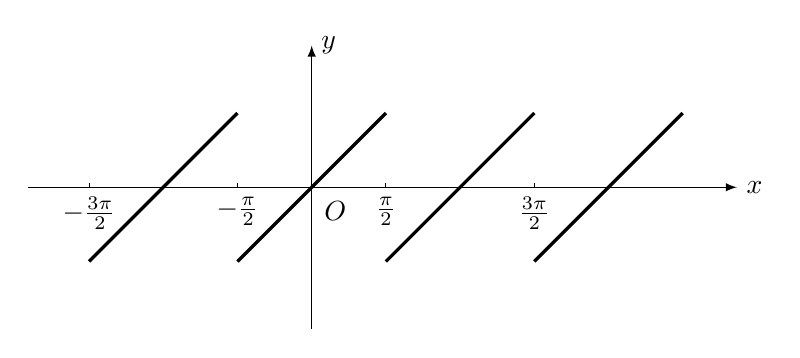
\begin{tikzpicture}[>=latex,scale=.6]
\draw[->] (-6,0)--(9,0)node[right]{$x$};
\draw[->] (0,-3)--(0,3)node[right]{$y$};    
\foreach \x/\xtext in {-1.5*pi/-\frac{3\pi}{2},-.5*pi/-\frac{\pi}{2},.5*pi/\frac{\pi}{2},1.5*pi/\frac{3\pi}{2}}
{
    \draw (\x,0)node[below]{$\xtext$}--(\x,.1);
}
\foreach \x in {-1.5*pi,-.5*pi,.5*pi,1.5*pi}
{
    \draw[very thick] (\x,-0.5*pi)--(\x+pi,0.5*pi);
}
\node at (.5,-.5){$O$};
\end{tikzpicture}
    \caption{}
\end{figure}
\end{solution}

\section{反余切函数}
由余切函数$y=\cot x$的图象可以看出函数$\cot x$在每个开区
间$(k\pi ,(k+1)\pi ),\; k\in\mathbb{Z}$内,由$+\infty$递减到$-\infty$, 所以在
每个这样的开区间里,反函数是存在的。

\begin{blk}{定义4}
     函数$y=\cot x$在开区间$(0,\pi )$内的反函数叫
\textbf{反余切函数或反余切},记作
\[x=\arctan y\]
它的定义域是开区间$-\infty<y<+\infty$。
\end{blk}


用几何名词来叙述反余切的定义便是:在开区间$-\infty<y<+\infty$内,数$y$的反余切
$x=\arccot y$
是开区间$0<x<\pi$ 内的一个角或弧,它的余切等于$y$, 即
$\cot x=y$。

由反余切的定义和反函数定理得到反余切的性质如下:
\begin{enumerate}
    \item $\arccot (\cot x)=x,\; 0<x<\pi ,\qquad 
\cot (\arccot y)=y,\; -\infty<y<+\infty$
\item 反余切是递减的函数并且连续;
\item $\arccot (-x)=\pi -\arccot x$。

这是因为
$\arccot x$和$\arccot (-x)$都属于$(0,\pi )$内的角,且
\[0=\pi -\pi <\pi - \arccot x<0+\pi =\pi \]
又
$\cot (\pi -\arccot x)=-\cot (\arccot x)=-x$,
所以
\[\pi -\arccot x=\arccot (-x)\]
即
\[\arccot (-x)=\pi -\arccot x\]
\item 反余切$y=\arccot x,\; -\infty<x<+\infty$的图象如图
9.11所示。
\end{enumerate}

\begin{figure}[htp]
    \centering
\begin{tikzpicture}[>=latex, scale=.8]
\draw[->] (-5,0)--(6,0)node[right]{$x$};
\draw[->] (0,-1)--(0,5)node[right]{$y$};
\draw (-5,pi)--(5,pi);
\node at (.25,-.25){$O$};
\node at (.2,pi)[above]{$\pi$};
\node at (.2,0.5*pi)[above]{$\frac{\pi}{2}$};
\draw [domain=.01:5, samples=100, very thick]plot(\x,{atan(1/\x)*pi/180});
\draw [domain=-5:-.01, samples=100, very thick]plot(\x,{atan(1/\x)*pi/180+pi});
\node at (-3.5,2.5){$y=\arccot x$};
\end{tikzpicture}    
    \caption{}
\end{figure}



\begin{example}
    求下列各式的值:(口答)
\begin{multicols}{2}
\begin{enumerate}
    \item $\arccot 1$
    \item $\arccot (- 1)$
    \item $\arccot \sqrt{3}$
    \item $\arccot \left(-\sqrt{3}\right)$
\end{enumerate}
\end{multicols}
\end{example}

\begin{solution}
\begin{enumerate}
    \item $\arccot 1=\frac{\pi}{4}$,因为$\cot\frac{\pi}{4}=1$,而且$0<\frac{\pi}{4}<\pi$。
    \item $\arccot (- 1)=\pi-\arccot 1=\pi-\frac{\pi}{4}=\frac{3\pi}{4}$
    \item $\arccot \sqrt{3}=\frac{\pi}{6}$,因为$\cot\frac{\pi}{6}=\sqrt{3}$,而且$0<\frac{\pi}{6}<\pi$。
    \item $\arccot \left(-\sqrt{3}\right)=\pi-\arccot\sqrt{3}=\pi-\frac{\pi}{6}=\frac{5\pi}{6}$
\end{enumerate}
\end{solution}


\begin{example}
    求$\sin\left[\arccot\left(-\frac{1}{3}\right)\right]$的值
\end{example}

\begin{solution}
    设$\arccot\left(-\frac{1}{3}\right)=\alpha$,其中$0<\alpha<\pi$,那么$\cot\alpha=-\frac{1}{3}$。

    由于$0<\alpha<\pi$,$\cot\alpha<0$,可以知道$\frac{\pi}{2}<\alpha<\pi$
\[\begin{split}
    \csc\alpha&=\sqrt{1+\cot^2\alpha}=\sqrt{1+\frac{1}{9}}=\sqrt{\frac{10}{9}}=\frac{\sqrt{10}}{3}\\
    \sin\alpha&=\frac{1}{\csc\alpha}=\frac{3}{\sqrt{10}}
\end{split}\]
$\therefore\quad \sin\left[\arccot\left(-\frac{1}{3}\right)\right]=\sin\alpha=\frac{3}{\sqrt{10}}=\frac{3\sqrt{10}}{10}$
\end{solution}


\begin{example}
    求证:对于任何实数$x$有
\[\arctan x+\arccot x=\frac{\pi}{2}\]
\end{example}

\begin{solution}
    设$\arctan x=\alpha$,其中$-\frac{\pi}{2}<\alpha<\frac{\pi}{2}$,则$\tan\alpha=x$。

    又$\cot\left(\frac{\pi}{2}-\alpha\right)=\tan\alpha=x$,而$0<\frac{\pi}{2}-\alpha<\pi$,所以$\frac{\pi}{2}-\alpha=\arccot x$。

    将$\alpha=\arctan x$代入上式,得到
    \[\frac{\pi}{2}-\arctan x=\arccot x\]
    所以:$\arctan x+\arccot x=\frac{\pi}{2},\quad x\in\mathbb{R}$
\end{solution}


\begin{example}
    证明$\arctan 3+\arccot\left(-\frac{1}{5}\right)=\pi-\arctan\frac{1}{8}$
\end{example}

\begin{solution}
设$\alpha=\arctan 3$,其中$0<\alpha<\frac{\pi}{2}$,则$\tan\alpha=3$。

又设$\beta=\arccot\left(-\frac{1}{5}\right)$,其中$\frac{\pi}{2}<\beta<\pi$,则:
\[\cot\beta=-\frac{1}{5},\qquad \tan\beta=-5\]
\[\begin{split}
 \tan\left[\arctan 3+\arccot\left(-\frac{1}{5}\right)\right]
&=\tan(\alpha+\beta)\\
&=\frac{\tan\alpha+\tan\beta}{1-\tan\alpha\cdot \tan\beta}\\
&=\frac{3+(-5)}{1-3(-5)}=-\frac{1}{8}
\end{split}\]
而且$\frac{\pi}{2}<\alpha+\beta<\frac{3\pi}{2}$,
\[\therefore\quad \arctan 3+\arccot\left(-\frac{1}{5}\right)=\arctan\left(-\frac{1}{8}\right)+\pi=\pi-\arctan\frac{1}{8}\]
\end{solution}

\section*{习题9.3}
\addcontentsline{toc}{subsection}{习题9.3}
\begin{enumerate}
    \item 用反三角函数表示下面等式中的角。
\begin{multicols}{2}
\begin{enumerate}
    \item $\tan\left(-\frac{\pi}{4}\right)=-1$
    \item $\tan\left(\frac{7\pi}{4}\right)=-1$
    \item $\tan\left(\frac{5\pi}{6}\right)=-\frac{1}{\sqrt{3}}$
    \item $\tan\left(-\frac{3\pi}{4}\right)=1$
    \item $\cot\frac{\pi}{6}=\sqrt{3}$
    \item $\cot\left(-\frac{5\pi}{4}\right)=-1$
    \item $\cot\left(-1\right)=-0.6421$
\end{enumerate}
\end{multicols}

\item 指出下列各函数哪些是偶函数?哪些是奇函数?哪
些既不是奇函数也不是偶函数。
\begin{multicols}{2}
    \begin{enumerate}
    \item $y=\arcsin x+2 \arctan x$
    \item $y=\arccos x+\arctan x$
    \item $y=\frac{\arcsin x}{\arccos x}$
    \item $y=\frac{\arctan x}{x}-x \arcsin x$
    \end{enumerate}
    \end{multicols}

    \item 计算下列各式的值:
\begin{multicols}{2}
\begin{enumerate}
\item  $\cos [\arctan(-\sqrt{3})]$;
\item  $\sin (\arctan 2)$;
\item $\arctan(\tan2)$
\item  $\arctan(\tan0.7 \pi)$
\item $\tan\left(\arctan \frac{1}{4}-\arccot  5\right)$
\item $\sin \left(\arctan \frac{8}{15}-\arcsin \frac{7}{18}\right)$
\item $\tan\left[2 \arctan\left(-\frac{1}{2}\right)\right]$
\item $\cos \left[2 \arctan \frac{1}{4}+\arccos \frac{3}{5}\right]$
\end{enumerate}
\end{multicols}

\item 检验下列各等式是否正确。
 \begin{enumerate}
\item $\arcsin \frac{15}{17}=\arccos \frac{8}{17}$
\item $\arcsin \frac{4}{5}=\arccot\frac{3}{4}$
\item $\arcsin \left(-\frac{7}{25}\right)=-\arctan \frac{7}{24}$
\item $\arccos \left(-\frac{9}{41}\right)=\pi-\arcsin \frac{40}{41}$
\item  $\arctan \frac{2}{3}+\arctan \frac{1}{5}=\frac{\pi}{4}$
\item $\arccot\frac{1}{9}+\arccot\frac{4}{5}=\frac{3}{4} \pi$
\item  $2 \arctan \frac{1}{3}+\arctan \frac{1}{4}=\arctan \frac{16}{13}$
\item $\arcsin \frac{7}{25}+\frac{1}{2} \arccos \frac{7}{25}=\arccos \frac{3}{5}$
\end{enumerate}   

\item 证明下面恒等式:
\begin{enumerate}
    \item 若$0<x<1$, 那么
\[\arcsin x=\arccos\sqrt{1-x^2}=\arctan\frac{x}{\sqrt{1-x^2}}=\arccot\frac{\sqrt{1-x^2}}{x}\]
    \item 若$0<x<1$, 那么
    \[\arccos x=\arcsin\sqrt{1-x^2}=\arctan\frac{\sqrt{1-x^2}}{x}=\arccot\frac{x}{\sqrt{1-x^2}}\]
    \item 若$x>0$, 那么
  \[\arctan x=\arccot \frac{1}{x}=\arcsin\frac{x}{\sqrt{1+x^2}}=\arccos\frac{1}{\sqrt{1+x^2}}\]
  \item 若$x>0$, 那么
  \[\arccot x=\arctan \frac{1}{x}=\arcsin\frac{1}{\sqrt{1+x^2}}=\arccos\frac{x}{\sqrt{1+x^2}}\]
  \item 若$|x|\le 1$,那么 $\arcsin x=\arctan\frac{x}{\sqrt{1-x^2}}$
  
  若$-1\le x\le 0$,那么 $\arcsin x=-\arccos{\sqrt{1-x^2}}$

  若$-1\le x< 0$,那么 $\arcsin x=\arctan\frac{\sqrt{1-x^2}}{x}-\pi$

\item 若$-1\le x\le 0$,那么 $\arccos x=\pi-\arcsin{\sqrt{1-x^2}}$

若$-1\le x< 0$,那么 $\arccos x=\pi+\arctan\frac{\sqrt{1-x^2}}{x}$

若$|x|\le 1$,那么 $\arccos x=\arctan\frac{x}{\sqrt{1-x^2}}$

\item 若$x<0$, 那么$\arctan x=\arccot \frac{1}{x}-\pi$

若$x<0$, 那么$\arccot x=\pi+\arctan\frac{1}{x}$

\item 若$x\ge 0$,$\frac{1}{2}\arccos(2x^2-1)=\arccos x$
\item 若$x\ge 1$,$2\arctan x+\arcsin\frac{2x}{1+x^2}=\pi$
\end{enumerate}

\item 作函数$y=x-\arctan(\tan x)$的草图。

\item 解下列方程:
\begin{enumerate}
    \begin{multicols}{2}
    \item $\arctan x=\frac{\pi}{4}$
    \item $\arctan x=\frac{\pi}{2}$
    \item $\arctan x=-\frac{\pi}{2}$
    \item $\arctan x^2=3$
    \item $\arctan 2x+\arctan 3x=\frac{3\pi}{4}$
\end{multicols}
    \item $\sin\Big\{2\arccos\big[\cot(2\arctan x)\big]\Big\}=0$
\end{enumerate}

\item 若$\arctan x+\arctan y+ \arctan z=\pi$, 
求证:$x+y+z=xyz$。

\item 求证:
\[\arctan x+\arctan\frac{1-x}{1+x}=\begin{cases}
    \frac{\pi}{4},& x>-1\\
    -\frac{3\pi}{4},& x<-1
\end{cases}\]
\end{enumerate}

\section{最简单的三角方程}
下列方程
$\sin x=a$, $\cos x=a$, $\tan x=a$, $\cot x=a$中的$a$为已给的
实数,$x$是未知数,是最简单的三角方程。适合其中某
个方程的$x$值叫做这个方程的解或根。例如,诸角:$x=
30^{\circ}$; $x=150^{\circ}$; $x=390^{\circ}$; $x=510^{\circ}$等等,为三角方程
$\sin x=\frac{1}{2}$
的解,因为,\[\sin30^{\circ}=\sin150^{\circ}=\sin390^{\circ}=\sin510^{\circ}=\frac{1}{2}\]

解三角方程就是求它的一切解,根据前一节内容知道,
已知三角函数值$a$所对应的角的值,如果存在的话,有无穷
多个,所以每一个三角方程都有无穷多个解,它的所有解简
称为通解。

在本节中,我们来解上面所示的最简单三角方程,从以
后的例子即将明白,解三角方程归根到底化为解最简单的
三角方程。

\subsection{最简单三角方程的解}
\subsubsection{$\sin x=a$的解}
分$|a|\le 1$和$|a|>1$的情形来考虑:

\textbf{第一种情形:} $0<a<1$
 
在坐标系$x$-$O$-$y$中,以原点$O$为圆心作一单位圆,在$Oy$
轴上作出纵坐标等于$a$的$Q$点,并过$Q$点引平行于$Ox$轴的直
线,交单位圆周于$A$和$B$二点,如图9.12, $P_0$为$(1,0)$,
$\angle P_0OA=\arcsin a$和$\angle P_0OB=\pi-\arcsin a$的正弦都等于$a$,
所以$\arcsin a$ 和$\pi-\arcsin a$是方程$\sin x=a$的特解,为求方程
$\sin x=a$的通解,可将$2k\pi$加于此两角中的每一个而得到,其
中$k\in\mathbb{Z}$. 因此,原方程的通解是
\[\begin{split}
   x_1&=2k\pi +\arcsin a\\
x_2&=2k\pi +\pi -\arcsin a=(2k+1)\pi -\arcsin a 
\end{split}\]
合并起来,可写成
\[x=k\pi +(-1)^k\arcsin a,\qquad k\in\mathbb{Z}\]

我们约定,在三角方程的通解中,“$k\in\mathbb{Z}$”以后不再
交代。

\begin{figure}[htp]\centering
    \begin{minipage}[t]{0.48\textwidth}
    \centering
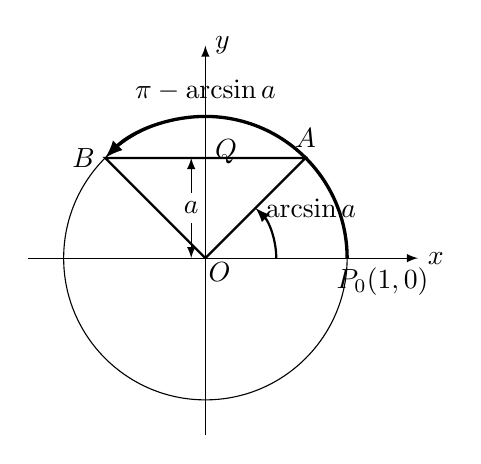
\begin{tikzpicture}[>=latex, scale=.9]
\draw [<->](-.2,0)--node[fill=white]{$a$}(-.2,1.414);
\draw[->] (-2.5,0)--(3,0)node[right]{$x$};
\draw[->] (0,-2.5)--(0,3)node[right]{$y$};
\draw (0,0) circle (2);
\draw[thick] (0,0)--(45:2)node[above]{$A$}--(135:2)node[left]{$B$}--(0,0);
\node at (.2,-.2){$O$};
\node at (0,1.5)[right]{$Q$};
\node at (2.5,0)[below]{$P_0(1,0)$};
\draw[->,  thick] (1,0) arc (0:45:1)node[right]{$\arcsin a$};
\draw[->, very thick] (2,0) arc (0:135:2);
\node at (0,2)[above=2pt]{$\pi-\arcsin a$};
    \end{tikzpicture}
    \caption{}
    \end{minipage}
    \begin{minipage}[t]{0.48\textwidth}
    \centering
    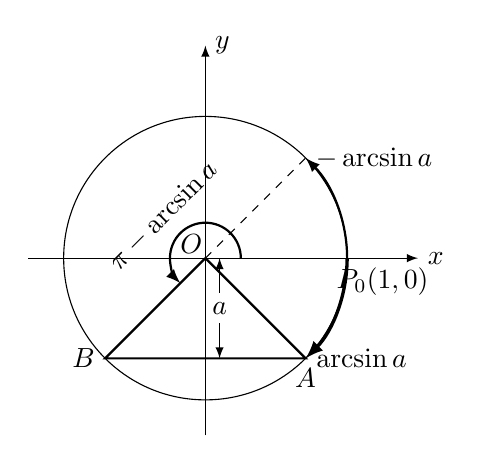
\begin{tikzpicture}[>=latex, scale=.9]
\draw [<->](.2,0)--node[fill=white]{$a$}(.2,-1.414);
\draw[->] (-2.5,0)--(3,0)node[right]{$x$};
\draw[->] (0,-2.5)--(0,3)node[right]{$y$};
\draw (0,0) circle (2);
\node at (-.2,.2){$O$};
\node at (2.5,0)[below]{$P_0(1,0)$};
\draw[thick] (0,0)--(-45:2)node[below]{$A$}--(-135:2)node[left]{$B$}--(0,0);
\draw[dashed] (0,0)--(45:2);
\draw[->, thick] (2,0) arc (0:45:2)node[right]{$-\arcsin a$};
\draw[->, very thick] (2,0) arc (0:-45:2)node[right]{$\arcsin a$};
\draw[->, thick] (.5,0) arc (0:180+45:.5);
\node at (-.6,.6)[rotate=45]{$\pi-\arcsin a$};

    \end{tikzpicture}
    \caption{}
    \end{minipage}
    \end{figure}


\textbf{第二种情形:} $-1<a<0$

用同样的方法作图,如图9.13所示:
$\angle P_0OA=\arcsin a$和$\angle P_0OB=\pi-\arcsin a$是方程$\sin x=a,\; -1<a<0$的特解,因此,原方程的通解仍是
\[\begin{split}
  x_1&=2k\pi +\arcsin a\\
x_2&=2k\pi +\pi -\arcsin a=(2k+1)\pi -\arcsin a  
\end{split}\]
合并起来,可写成
\[x=k\pi +(-1)^k\arcsin a\]

\textbf{第三种情形:} $a=1$

方程$\sin x=1$的特解是$x=\frac{\pi}{2}$,
因此,原方程的通解是
\[x=\frac{\pi}{2}+2k\pi\quad \text{或者}\quad x=90^{\circ}+k\cdot 360^{\circ}\]

\textbf{第四种情形:} $a=-1$

\[\sin x=-1\]
特解:$x=-\frac{\pi}{2}$(或$x=-90^{\circ}$),

通解:$x=-\frac{\pi}{2}+2k\pi$ (或$x=-90^{\circ}+k\cdot 360^{\circ}$)。

\textbf{第五种情形:} $a=0$

\[\sin x=0\]
特解:$x_1=0$和$x_2=\pi$。

通解:$x_1=2k\pi$和$x_2=\pi +2k\pi =(2k+1)\pi$,
合并成:\[x=k\pi\]

\textbf{第六种情形:} $|a|>1$

在这种情形下,$\sin x=a$没有解。

将结果总结于下表内
\begin{center}
\begin{tabular}{c|c}
    \hline
$a$的数值& 方程$\sin x=a$的解\\
    \hline
$-1<a<0,\; 0<a<1$ & $x=k\pi +(-1)^k\arcsin a$\\
$a=-1$& $x=-\frac{\pi}{2}+2k\pi$\\
$a=0$&   $x=k\pi$\\
$a=1$& $x=\frac{\pi}{2}+2k\pi$\\
$|a|>1$ & 方程无解\\
    \hline
\end{tabular}   
\end{center}

\begin{example}
    解方程$\sin x=\frac{1}{2} $
\end{example}

\begin{solution}
    \[x=k\pi+(-1)^k\arcsin\frac{1}{2}=k\pi+(-1)^k\frac{\pi}{6}\]
    或者\[x=k\cdot 360^{\circ}+(-1)^k\cdot 30^{\circ},\qquad (k\in\mathbb{Z})\]
\end{solution}


\begin{example}
    解方程$\sin x=-\frac{1}{2} $
\end{example}

\begin{solution}
\[x=k\pi+(-1)^k\arcsin\left(-\frac{1}{2}\right)=k\pi+(-1)^{k+1}\frac{\pi}{6}\]
    或者\[x=k\cdot 360^{\circ}+(-1)^{k+1}\cdot  30^{\circ},\qquad (k\in\mathbb{Z})\]
\end{solution}


\begin{example}
    解方程$\sin (2x-1)=\frac{\sqrt{3}}{2} $
\end{example}

\begin{solution}
\[\begin{split}
   2x-1&=k\pi+(-1)^k \arcsin\frac{\sqrt{3}}{2}\\ 
2x&=k\pi+(-1)^k \cdot \frac{\pi}{3}+1\\
  x &=k\cdot\frac{\pi}{2}+(-1)^k\cdot \frac{\pi}{6}+\frac{1}{2} ,\qquad (k\in\mathbb{Z})
 \end{split}\]   
\end{solution}

\subsubsection{$\cos x=a$的解}

\textbf{第一种情形:} $0<a<1$
在$Ox$轴上作出横坐标等于$a$的$P$点,并过$P$点作平行于$Oy$
轴的直线交单位圆周于$C$和$D$二点,$P_0$为$(1,0)$(图9.14)。
$\angle P_0OC=\arccos a$和$\angle P_0OD=-\arccos a$的余弦等于$a$, 故它
们是方程的解,原方程的通解是
\[x=2k\pi\pm \arccos a\]

\textbf{第二种情形:} $-1<a<0$
作类似的图形,如图9.15同样可得原方程的通解是
\[x=2k\pi\pm \arccos a\]

\begin{figure}[htp]\centering
    \begin{minipage}[t]{0.48\textwidth}
    \centering
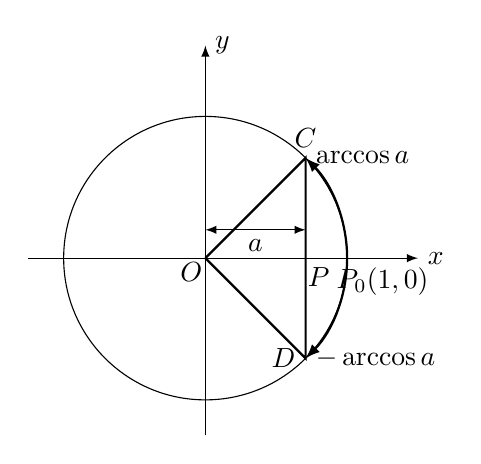
\begin{tikzpicture}[>=latex, scale=.9]
\draw [<->](0,.4)--node[below]{$a$}(1.414,.4);
\draw[->] (-2.5,0)--(3,0)node[right]{$x$};
\draw[->] (0,-2.5)--(0,3)node[right]{$y$};
\draw (0,0) circle (2);
\draw[thick] (0,0)--(45:2)node[above]{$C$}--(-45:2)node[left]{$D$}--(0,0);
\node at (-.2,-.2){$O$};
\node at (1.6,0)[below]{$P$};
\node at (2.5,0)[below]{$P_0(1,0)$};
\draw[->,  thick] (2,0) arc (0:45:2)node[right]{$\arccos a$};
\draw[->,  thick] (2,0) arc (0:-45:2)node[right]{$-\arccos a$};
    \end{tikzpicture}
    \caption{}
    \end{minipage}
    \begin{minipage}[t]{0.48\textwidth}
    \centering
    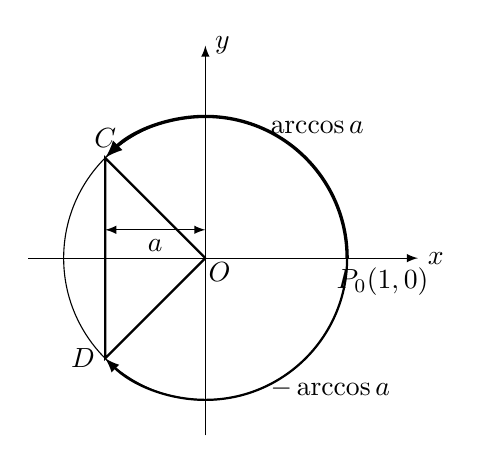
\begin{tikzpicture}[>=latex, scale=.9]
\draw [<->](0,.4)--node[below]{$a$}(-1.414,.4);
\draw[->] (-2.5,0)--(3,0)node[right]{$x$};
\draw[->] (0,-2.5)--(0,3)node[right]{$y$};
\draw (0,0) circle (2);
\draw[thick] (0,0)--(135:2)node[above]{$C$}--(-135:2)node[left]{$D$}--(0,0);
\node at (.2,-.2){$O$};
\node at (2.5,0)[below]{$P_0(1,0)$};
\draw[->, very thick] (2,0) arc (0:135:2);
\draw[->,  thick] (2,0) arc (0:-135:2);
\node at (67:2)[right]{$\arccos a$};
\node at (-67:2)[right]{$-\arccos a$};
    \end{tikzpicture}
    \caption{}
    \end{minipage}
    \end{figure}

\textbf{第三种情形:} $a=1$

\[\cos x=1\]

方程的特解:$x=0$, 方程的通解:$x=2k\pi$。

\textbf{第四种情形:} $a=-1$

\[\cos x=-1\]
方程的特解:$x=\pi$, 方程的通解:$x=\pi+2k\pi=(2k+1)\pi$。

\textbf{第五种情形:} $a=0$
\[\cos x=0\]
方程的特解:$x_1=\frac{\pi}{2}$和$x_2=-\frac{\pi}{2}=\frac{\pi}{2}-\pi$。

方程的通解:$x=\frac{\pi}{2}+k\pi$。

\textbf{第六种情形:} $|a|>1$

在这种情形下,方程$\cos x=a$无解。

将结果综合于下表内:
\begin{center}
    \begin{tabular}{c|c}
        \hline
    $a$的数值& 方程$\cos x=a$的解\\
        \hline
    $-1<a<0,\; 0<a<1$ & $x=2k\pi \pm \arccos a$\\
    $a=-1$& $x=(2k+1)\pi$\\
    $a=0$&   $x=\frac{\pi}{2}+k\pi$\\
    $a=1$& $x=2k\pi$\\
    $|a|>1$ & 方程无解\\
        \hline
    \end{tabular}   
    \end{center}



\begin{example}
    解方程$2\cos x+1=0$
\end{example}

\begin{solution}
    化简为$\cos x=-\frac{1}{2}$,通解如下:
\[\begin{split}
    x&=2k\pi\pm\arccos\left(-\frac{1}{2}\right)\\
    &=2k\pi\pm \left(\pi-\arccos\frac{1}{2}\right)\\
    &=2k\pi\pm \left(\pi-\frac{\pi}{3}\right)\\
    &=2k\pi\pm \frac{2\pi}{3}
\end{split}\]
\end{solution}


\begin{example}
    解方程$\cos\left(\frac{x}{4}+\frac{\pi}{5}\right)=0$
\end{example}

\begin{solution}
    \[\begin{split}
        \frac{x}{4}+\frac{\pi}{5}&=\frac{\pi}{2}+k\pi\\
        \frac{x}{4}&=\frac{\pi}{2}-\frac{\pi}{5}+k\pi=\frac{3\pi}{10}+k\pi\\
        x&=4\left(\frac{3\pi}{10}+k\pi\right)=\frac{6\pi}{5}+4k\pi
    \end{split}
    \]
\end{solution}

\subsubsection{$\tan x=a$的解}

如图9.16所示,$\angle P_0OA=\arctan a$和$\angle P_0OB=\pi+\arctan a$
是方程的解,因为它们的正切
等于$a$. 原方程的通解是
\[x=k\pi+\arctan a\]


\begin{example}
    解方程$\tan x=-1$    
\end{example}

\begin{solution}
\[x=k\pi+\arctan(-1)=k\pi-\arctan1=k\pi-\frac{\pi}{4}\]
\end{solution}

\subsubsection{$\cot x=a$的解}

如图9.17所示,$\angle P_0OA=\arccot a$和$\angle P_0OB=\pi+\arccot a$是方
程的特解,因为它们的余切等于$a$. 原方程的通解是
\[x=k\pi+\arccot a,\qquad (k\in\mathbb{Z})\]

\begin{figure}[htp]\centering
    \begin{minipage}[t]{0.48\textwidth}
    \centering
\begin{tikzpicture}[>=latex, scale=.9]
\draw [|<->|](2.2,0)--node[right]{$a$}(2.2,2);
\draw[->] (-2.5,0)--(3,0)node[right]{$x$};
\draw[->] (0,-2.5)--(0,3)node[right]{$y$};
\draw (0,0) circle (2);
\draw[thick] (-135:2)node[below]{$B$}--(0,0)--(45:2)node[above]{$A$}--(2,2);
\node at (.2,-.2){$O$};
\node at (2.7,0)[below]{$P_0(1,0)$};
\draw[->, very thick] (2,0) arc (0:45:2);
\draw[->,  thick] (2,0) arc (0:180+45:2);
\node at (1,.3){$\arctan a$};
\node at (-2,1.5){$\pi+\arctan a$};
\draw(2,-2.5)--(2,3)node[right]{正切线};
    \end{tikzpicture}
    \caption{}
    \end{minipage}
    \begin{minipage}[t]{0.48\textwidth}
    \centering
    \begin{tikzpicture}[>=latex, scale=.9]
\draw [|<->|](0,2.2)--node[above]{$a$}(2,2.2);
\draw[->] (-2.5,0)--(3,0)node[right]{$x$};
\draw[->] (0,-2.5)--(0,3)node[right]{$y$};
\draw (0,0) circle (2);
\draw[thick] (-135:2)node[below]{$B$}--(0,0)--(45:2)node[above]{$A$}--(2,2);
\node at (.2,-.2){$O$};
\node at (2.7,0)[below]{$P_0(1,0)$};
\draw[->, very thick] (2,0) arc (0:45:2);
\draw[->,  thick] (2,0) arc (0:180+45:2);
\node at (23:2.2)[right]{$\arccot a$};
\node at (-2,1.5){$\pi+\arccot a$};
\draw(-2.5,2)--(3,2)node[above]{余切线};
    \end{tikzpicture}
    \caption{}
    \end{minipage}
    \end{figure}


\begin{example}
    解方程$9\cot^2 2x-25=0$
\end{example}

\begin{solution}
    \[\begin{split}
        \cot^2 2x&=\frac{25}{9}\\
        \cot 2x&=\pm\frac{5}{3}\approx \pm 1.6667
    \end{split}\]
由$\cot 2x=1.6667$,得:
\[\begin{split}
    2x&=30^{\circ}58'+k\cdot 180^{\circ}\\
    x&=15^{\circ}29'+k\cdot 90^{\circ}
\end{split}\]
由$\cot 2x=-1.6667$,得:
\[\begin{split}
    2x&=(180^{\circ}-30^{\circ}58')+k\cdot 180^{\circ}\\
    2x&=149^{\circ}2'+k\cdot 180^{\circ}\\
    x&=74^{\circ}31'+k\cdot 90^{\circ}
\end{split}\]
$\therefore\quad $原方程的近似解是:
\[x=15^{\circ}29'+k\cdot 90^{\circ}\quad \text{和}\quad x=74^{\circ}31'+k\cdot 90^{\circ}\]
\end{solution}

\subsection{解简单三角方程的例子}
在本节中,我们来研究某些三角方程的解法。解这些方
程时,一般是应用三角函数的恒等变形和解代数方程的一般
知识把它归结成解一个或几个最简单的三角方程,从而求出
所有解。在解三角方程的过程中,应当避免作可能破坏方程
同解性的变形,如果这类变形不可避免,则需研究哪些根会失
掉,哪些根是增根,对最终方程的诸解,应当进行检验,确
定它们是否是原方程的解。下面通过例子来阐明。

\subsubsection{含有同角的同名三角函数的方程}
\begin{example}
    解方程
 $   2\cos^2x+\cos x-1=0$
\end{example}

\begin{solution}
    把方程看作关于未知数为$\cos x$的二次方程,按照二
次方程的解法,可得
\[\cos x=\frac{-1\pm\sqrt{1+8}}{4}=\frac{-1\pm 3}{4}\]
由此得:$\cos x=\frac{1}{2}$或$\cos x=-1$。

由$\cos x=\frac{1}{2}$,得:$x=2k\pi+\frac{\pi}{3}$;由$\cos x=-1$,得:$x=(2k+1)\pi$。

$\therefore\quad $原方程的解集是
\[\left\{x\big| x=2k\pi\pm \frac{\pi}{3}\right\}\cup \left\{x\big| x=(2k+1)\pi \right\}\]
\end{solution}

\begin{example}
    解方程$2\sin^2x+2\sin x-\sqrt{3}\sin x=\sqrt{3}$
\end{example}

\begin{solution}
\textbf{解法1:} 把一切项都移至左端,得:$2\sin^2x+\left(2-\sqrt{3}\right)\sin x-\sqrt{3}=0$
解关于$\sin x$的二次方程,得
\[\begin{split}
\sin x&=\frac{-2+\sqrt{3}\pm \sqrt{\left(2-\sqrt{3}\right)^2+8\sqrt{3}}}{4}\\
&=\frac{-2+\sqrt{3}\pm \sqrt{4+4\sqrt{3}+3}}{4}\\
&=\frac{-2+\sqrt{3}\pm \sqrt{\left(2+\sqrt{3}\right)^2}}{4}\\
&=\frac{-2+\sqrt{3}\pm \left(2+\sqrt{3}\right)}{4}
\end{split}\]
由此得
\[\sin x=\frac{\sqrt{3}}{2}\quad \text{或}\quad \sin x=-1\]

由$\sin x=\frac{\sqrt{3}}{2}$得:$x=k\cdot 180^{\circ}+(-1)^k\cdot 60^{\circ}$。

由$\sin x=-1$得:$x=-90^{\circ}+k\cdot 360^{\circ}$。

$\therefore\quad $原方程的解集是
\[\left\{x|x=k\cdot 180^{\circ}+(-1)^k\cdot 60^{\circ}\right\}\cup \left\{x|x=-90^{\circ}+k\cdot 360^{\circ}\right\}\]
这里$k\in\mathbb{Z}$。

\textbf{解法2:} 把一切项都移至左端得:$2\sin^2x+2\sin x-\sqrt{3}\sin x-\sqrt{3}=0$

方程左端可以分解因式:
\[\begin{split}
    2\sin x(\sin x+1)-\sqrt{3}(\sin x+1)&=0\\
    (\sin x+1)\left(2\sin x-\sqrt{3}\right)&=0
\end{split}\]

若两个因式的乘积等于零,则至少有一个因式等于零,
同时应当满足下列条件:对于使第一个因式为零的解,应当
使方程的第二个因式有确定的值。上面的方程可分为这样的
两个方程:
\[2\sin x-\sqrt{3}=0\quad \text{或}\quad \sin x+1=0\]
分别由$\sin x=\frac{\sqrt{3}}{2} $和$\sin x=-1$,得到:
\[x=k\pi+(-1)^k \cdot\frac{\pi}{3}\quad \text{和}\quad x=-\frac{\pi}{2}+2k\pi\]

把$x=k\pi+(-1)^k \cdot\frac{\pi}{3}$代入$\sin x+1$中,有确定值,同
样把$x=-\frac{\pi}{2}+2k\pi$代入$2\sin x-\sqrt{3}$中,也有确定值,所以
原方程的解集是
\[\left\{x\Big|x=k\pi+(-1)^k \cdot\frac{\pi}{3}\right\}\bigcup \left\{x\Big|x=-\frac{\pi}{2}+2k\pi\right\}\]
\end{solution}

一般的情况下,在三角方程中,不只有一个三角函数,
我们可以利用同一个角的各三角函数值之间的关系式,把方
程中未知角的各三角函数都用某一个三角函数表示出来,这
样,就把所解的三角方程先归结到多项式方程的问题。

\begin{example}
    解方程 $\sin^2 x+\cos x+1=0$
\end{example}

\begin{solution}
$\because\quad \sin^2 x=1-\cos^2x$,\qquad $\therefore\quad $原方程可化为:
\[\begin{split}
    \cos^2x-\cos x-2&=0\\
    \cos x&=\frac{1\pm 3}{2}
\end{split}\]
由此得到
\[\cos x=2\quad \text{或}\quad \cos x=-1\]

$\because\quad \cos x=2>1$,\qquad  $\therefore\quad $方程无解。

由$ \cos x=-1$,得:$x=(2k+1)\pi$

$\therefore\quad $原方程的解集是$\{x|x=(2k+1)\pi,\; k\in\mathbb{Z}\}$。
\end{solution}

\begin{example}
    解方程$\cos x-\sin x=0$
\end{example}

\begin{solution}
    如果用$\cos x$表示$\sin x$或用$\sin x$表示$\cos x$, 那么我们就
    得到根式方程,为了避免这点,可以用$\cos x$去除方程的两
    边,得到
    \[1-\tan x=0\]
    因为原方程的解不含有$\cos x=0$的解,所以我们有根据这样
    做。事实上,由$\cos x=0$, 得到
    $x=\frac{\pi}{2}+k\pi$, 代入$\cos x-\sin x$中,有
   \[ \cos\left(\frac{\pi}{2}+k\pi \right)-sin\left(\frac{\pi}{2}+k\pi \right)=0-(-1)^k\sin \frac{\pi}{2}=(-1)^{k+1}\ne 0\]
    不满足原方程。
    
    因此,用$\cos x$去除原方程的两边,得到和原方程同解的方程
    \[\tan x=1\]
    由此,
   $ x=k\pi +\frac{\pi}{4}$。

   所以原方程的解集是
$\left\{x\Big|x=k\pi+\frac{\pi}{4},\; k\in\mathbb{Z}\right\}$
\end{solution}

\begin{rmk}
当解$\cos x-\sin x=0$时,也可以把
$\cos x$提出括号之外,而不用$\cos x$去除两端,原方程可写成下面的形式
$$\cos x (1-\tan x)=0$$
由此得到
$$\cos x=0\quad \text{或}\quad \tan x=1$$
但是使$\cos x=0$的解:$x=\frac{\pi}{2}+k\pi$却使因式$1-\tan x$无意义,这就表示$x=\frac{\pi}{2}+k\pi$是原方程的增根,因此必须舍去,同样我们得到原方程的同解方程
$\tan x=1$。

对于例9.29这种方程的解法还可以应用到下面更一般的类
型上去。

左端是关于$\sin x$和$\cos x$的齐次多项式右端是零的方程,
称为\textbf{齐次方程},例9.29的方程是齐次方程的一个特例。
\end{rmk}




\begin{example}
    解齐次方程$2\sin^2x-7\sin x\cos x+6\cos^2x=0$
\end{example}

\begin{solution}
用$\cos^2x$除原方程的两端,得
\[2\tan^2 x-7\tan x+6=0\]
由此得$\tan x=2\quad \text{或}\quad \tan x=1.5$

由$\tan x=2$得
\[x\approx k\cdot 180^{\circ}+63^{\circ}26'\]

由$\tan x=1.5$得
\[x\approx k\cdot 180^{\circ}+56^{\circ}19'\]
$\therefore\quad $原方程的解集是:
\[\left\{x\big|x=k\cdot 180^{\circ}+63^{\circ}26' \right\}\cup \left\{x\big|x=k\cdot 180^{\circ}+56^{\circ}19' \right\}\]
或者
\[\left\{x\big|x=k\pi+\arctan 2 \right\}\bigcup\left\{x\big|x=k\pi+\arctan\frac{3}{2} \right\}\]

又这样的方程
$2\sin^2x+5\sin x\cos x+\cos^2x=4$
也可以归入齐次方程,因为原方程可写成
\[2\sin^2x+5\sin x\cos x+\cos^2x-4(\cos^2x+\sin^2x)=0\]
化简得
\[2\sin^2x-5\sin x\cos x+3\cos^2x=0\]
\end{solution}

\begin{example}
    解方程$8\sin^2\frac{x}{2}+3\sin x-4=0$
\end{example}

\begin{solution}
    原方程可以变形为齐次方程
\[8\sin^2\frac{x}{2}+6\sin \frac{x}{2}\cos\frac{x}{2}-4\left(\sin^2\frac{x}{2}+\cos^2\frac{x}{2}\right)=0\]
化简得:$2\sin^2\frac{x}{2}+3\sin\frac{x}{2}\cos\frac{x}{2}-2\cos^2\frac{x}{2}=0$。

两边除以$\cos^2\frac{x}{2}$, 得
    \[2\tan^2\frac{x}{2}+3\tan\frac{x}{2}-2=0\]
所以$\tan\frac{x}{2}=-2\quad \text{或}\quad \tan\frac{x}{2}=\frac{1}{2}$。

由$\tan\frac{x}{2}=-2$得:
\[\begin{split}
    \frac{x}{2}&=-\arctan 2+k\pi\\
    x=-2\arctan 2+2k\pi
\end{split}\]

由$\tan\frac{x}{2}=\frac{1}{2}$得:
\[\begin{split}
    \frac{x}{2}&=\arctan \frac{1}{2}+k\pi\\
    x=2\arctan \frac{1}{2}+2k\pi
\end{split}\]
因为原方程的解不含有$\cos^2\frac{x}{2}=0$的解,所以,这样解不会
丢根,由此知原方程的解是
\[\left\{x\big|x=-2\arctan 2+2k\pi \right\}\cup \left\{x\big|x=2\arctan \frac{1}{2}+2k\pi \right\}\]
\end{solution}

\subsubsection{一边为零,另一边可以分解为因式的乘积的方程}
\begin{example}
    解方程
$1-\cos x =\tan x-\sin x$
\end{example}

\begin{solution}
    原方程可变形为:$1-\cos x =\tan x(1-\cos x)$

    如果方程的两边除以$1-\cos x$, 那么,原方程中就会丢掉$1-\cos x=0$的根。
为了不致丢掉这些根,把因式$1-\cos x$
提出,方程就变
形为:
\[(1-\cos x)(1-\tan x)=0\]
于是
$$1-\cos x=0\quad  \text{或}\quad 1-\tan x=0$$
由$\cos x=1$得到$x=2k\pi$, 由$\tan x=1$得到$x=\frac{\pi}{4}+k\pi$。

由于方程$\cos x=1$的解使因式$1-\tan x$有确定值,而方程
$\tan x=1$的解也使因式$1-\cos x$有确定值,所以原方程的解集是
\[\left\{x\big|x=2k\pi\right\}\cup \left\{x\big|x=\frac{\pi}{4}+k\pi\right\}\]
\end{solution}


\begin{example}
    解方程 $\tan x+\tan 2x-\tan 3x=0$
\end{example}

\begin{solution}
    原方程可写成
    $\tan 3x(1-\tan x\cdot \tan 2x)-\tan 3x=0$

    化简得:$\tan x\cdot \tan 2x\cdot \tan 3x=0$,由此得:
 \[ \tan  x=0 \quad \text{或}\quad \tan 2x=0 \quad \text{或}\quad \tan 3x=0\]
    由$\tan x=0$得$x=k\pi$;由$\tan 2x=0$得
    $x=\frac{k\pi}{2}$;由$\tan 3x=0$得$x=\frac{k\pi}{3}$
 
    把各方程的解标在单位圆上,得到满足各方程的角的终
    边,如图9.18所示。
\begin{figure}[htp]
    \centering
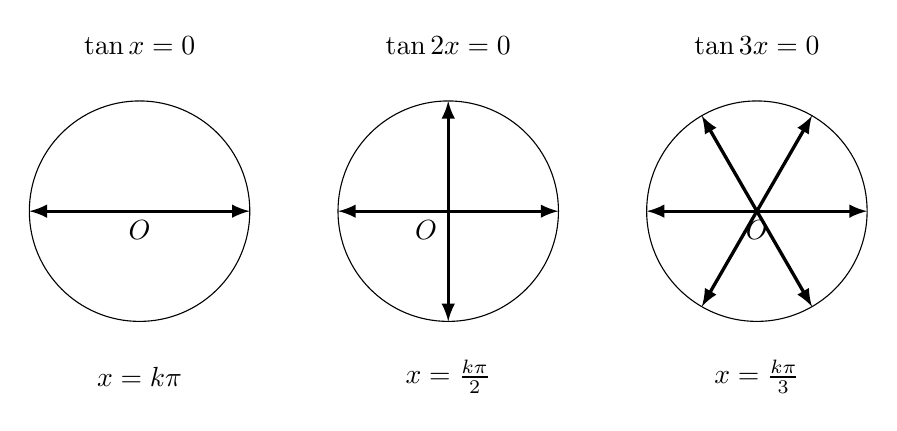
\begin{tikzpicture}[>=latex, scale=1.4]
\begin{scope}
    \draw (0,0) circle (1);
    \draw[<->, very thick] (0:1)--(180:1);
    \node at (0,0)[below]{$O$};
\node at (0,1.5){$\tan x=0$};
\node at (0,-1.5){$x=k\pi$};
\end{scope}
\begin{scope}[xshift=2.8cm]
    \draw (0,0) circle (1);
    \draw[<->, very thick] (0:1)--(180:1);
    \draw[<->, very thick] (90:1)--(-90:1);
    \node at (-.2,0)[below]{$O$};
\node at (0,1.5){$\tan 2x=0$};
\node at (0,-1.5){$x=\frac{k\pi}{2}$};
\end{scope}
\begin{scope}[xshift=5.6cm]
    \draw (0,0) circle (1);
    \draw[<->, very thick] (0:1)--(180:1);
    \draw[<->, very thick] (60:1)--(180+60:1);
    \draw[<->, very thick] (120:1)--(-60:1);
    \node at (0,0)[below]{$O$};
\node at (0,1.5){$\tan 3x=0$};
\node at (0,-1.5){$x=\frac{k\pi}{3}$};
\end{scope}
\end{tikzpicture} 
    \caption{}
\end{figure}

$\because\quad \tan x=0$的解$x=k\pi=3k\cdot \frac{\pi}{3}\in \{x|tan 3x=0\}=\left\{x\big| x=k\cdot \frac{\pi}{3}\right\}$

又$\tan 2x=0$的解$x=k\cdot \frac{\pi}{2}$
中,当$k=2n+1$时,使$\tan x$没有确定
值,必须舍去;又当$k=2n$时,
\[x=n\pi=3n\cdot \frac{\pi}{3}\in\left\{x\big|x=k\cdot \frac{\pi}{3}\right\}=\{x|\tan 3x=0\}\]
因此,所求方程的解集是
$\left\{x\big|x=k\cdot \frac{\pi}{3},\quad k\in\mathbb{Z}\right\}$
\end{solution}

\begin{example}
    解方程
$\sin x+\tan x=\sec x-\cos x$
\end{example}

\begin{solution}
两边同乘以$\cos x$, 得到
$\sin x\cos x+\sin x=1-\cos^2x$
移项,提取公因式得
\[\sin x(\cos x +1-\sin x)=0\]
由此得
\[\sin x=0\quad  \text{或}\quad \cos x+1-\sin x=0\]

由$\sin x=0$, 得$x=k\pi$. 

由$\sin x-\cos x=1$,变形为$\sin x-\sin(90^{\circ}-x)=1$,
即:
\[2\cos45^{\circ} sin\left(x-\frac{\pi}{4}\right)=1\]
即$\sin\left(x-\frac{\pi}{4}\right)=\frac{\sqrt{2}}{2}$

由此得:
\[x-\frac{\pi}{4}=\frac{\pi}{4}+2k\pi\quad  \text{或}\quad x-\frac{\pi}{4}=\frac{3\pi}{4}+2k\pi\]
即
\[x=\frac{\pi}{2}+2k\pi\quad  \text{或}\quad x=(2k+1)\pi\]
这样,我们由已知方程得到3组解:
\begin{align}
    x&=k\pi\\
    x&=\frac{\pi}{2}+2k\pi\\
    x&=(2k+1)\pi
\end{align}
因为$\{x|x=(2k+1)\pi\}\subset \{x|x=k\pi\}$,又$x=\frac{\pi}{2}+2k\pi$使$\cos x=0$,因此对于$x$的这些值,原方
程中的函数$\tan x$及$\sec x$无意义,这就是说$x=\frac{\pi}{2}+2k\pi$是增
根,必须舍去,所以原方程的解集是$\{x|x=k\pi,\; k\in\mathbb{Z}\}$。
\end{solution}

\begin{example}
    解方程$\sin7x=\sin5x$
\end{example}

\begin{solution}    
\textbf{解法1:}移项,得$\sin7x-\sin5x=0$,利用和差化积公式得
\[2\cos6x\sin x=0\]
由此得
\[\cos6x=0\quad  \text{或}\quad \sin x=0\]
由$\cos6x=0$,得:
\[\begin{split}
    6x&=\frac{\pi}{2}+k\pi\\
    x&=\frac{\pi}{12}+k\cdot \frac{\pi}{6}
\end{split} \]
由$\sin x=0$,得:$x=k\pi$。
    
所求方程的解集是
\[\left\{x\big|x=\frac{\pi}{12}+k\cdot \frac{\pi}{6}\right\}\cup\left\{x\big|x=k\pi\right\} \]
    
\textbf{解法2:} 利用二角正弦相等条件有
\[7x=5x+2k\pi \quad \text{或}\quad 7x=\pi -5x+2k\pi \]

由$7x=5x+2k\pi$得 $2x=2k\pi$,因此:$x=k\pi$。

由$7x=\pi -5x+2k\pi$得
$12x=\pi +2k\pi$, 因此:$x=\frac{\pi}{12}+k\cdot \frac{\pi}{6}$

$\therefore\quad $方程的解集是
\[\left\{x\big|x=k\pi\right\}\cup\left\{x\big|x=\frac{\pi}{12}+k\cdot \frac{\pi}{6}\right\} \]

我们得到与第一种解法相同的结果。
\end{solution}

\subsubsection{$a\sin x +b\cos x=c$型的方程}

\paragraph{第一种方法} 引入辅助角$\varphi$,让方程的两端除以$\sqrt{a^2+b^2}$, 得到
\[\frac{a}{\sqrt{a^{2}+b^{2}}} \sin x+\frac{b}{\sqrt{a^{2}+b^{2}}} \cos x=\frac{c}{\sqrt{a^{2}+b^{2}}}\]
令$\cos \varphi=\frac{a}{\sqrt{a^{2}+b^{2}}}, \quad \sin \varphi=\frac{b}{\sqrt{a^{2}+b^{2}}}$,
由点 $(a, b)$ 所在的象限定出角 $\varphi$ 是第几象限角, 可由 
$\tan \varphi=\frac{b}{a}$ 求出$\varphi$的值, 于是原方程可写成
\[\sin x \cos \varphi+\cos x \sin \varphi=\frac{c}{\sqrt{a^{2}+b^{2}}}\]
即 $\sin (x+\varphi)=\frac{c}{\sqrt{a^{2}+b^{2}}}$

解出 
\begin{equation}
    x+\varphi=2 k \pi+\arcsin \frac{c}{\sqrt{a^{2}+b^{2}}}
\end{equation}
或
\begin{equation}
    x+\varphi=2 k \pi+\pi-\arcsin \frac{c}{\sqrt{a^{2}+b^{2}}}
\end{equation}
由此得到
\[x=2 k \pi+\arcsin \frac{c}{\sqrt{a^{2}+b^{2}}}-\varphi\]
或
\[x=(2 k+1) \pi-\arcsin \frac{c}{\sqrt{a^{2}+b^{2}}}-\varphi\]

讨论:原方程有解的必要且充分条件是$\left| \frac{c}{\sqrt{a^{2}+b^{2}}}\right|\le 1$,即$\frac{c^2}{a^2+b^2}\le 1$,由此得到
$a^2+b^2\ge c^2$.

\begin{example}
    解方程$-\sqrt{3}\sin x+\cos x=1$
\end{example}

\begin{solution}
    原方程两边除以$\sqrt{(-\sqrt{3})^2+1}=2$, 得到
\[-\frac{\sqrt{3}}{2}\sin x+\frac{1}{2}\cos x=\frac{1}{2}\]
令$\cos\varphi=-\frac{\sqrt{3}}{2}<0,\quad \sin\varphi=\frac{1}{2}>0$,则角$\varphi$是第一象限角,
\[\varphi=\arccos\left(-\frac{\sqrt{3}}{2}\right)=\pi-\arccos\frac{\sqrt{3}}{2}=\pi-\frac{\pi}{6}=\frac{5\pi}{6}\]
于是,原方程可写成
\[\sin x\cos\frac{5\pi}{6}+\cos x\sin \frac{5\pi}{6}=\frac{1}{2}\]
即:$\sin\left(x+\frac{5\pi}{6}\right)=\frac{1}{2}$。

$\therefore\quad x+\frac{5\pi}{6}=2k\pi+\frac{\pi}{6}\quad \text{或}\quad x+\frac{5\pi}{6}=2k\pi+\left(\pi-\frac{\pi}{6}\right)$

由此:$x=2k\pi-\frac{2\pi}{3}\quad \text{或}\quad x=2k\pi$。

$\therefore\quad $原方程的解集是
\[\left\{x\big|x=2k\pi-\frac{2\pi}{3}\right\}\cup \left\{x\big|x=2k\pi\right\}\]
\end{solution}

\begin{example}
    解方程$2\sin x-3\cos x =\sqrt{13}$
\end{example}

\begin{solution}
方程两边除以$\sqrt{2^2+(-3)^2}=\sqrt{13}$, 得到
\[\frac{2}{\sqrt{13}}\sin x+\frac{(-3)}{\sqrt{13}}\cos x=1\]
令$\cos\varphi=\frac{2}{\sqrt{13}}>0,\quad \sin\varphi=\frac{-3}{\sqrt{13}}<0$则角$\varphi$是第四象限角,且由$\tan \varphi=-\frac{3}{2}=-1.5$, 查表得出
$\varphi=\arctan (-1.5)\approx -56^{\circ}18'$, 于是原方程可写成
\[\sin x\cos(-56^{\circ}18')+\cos x\sin(-56^{\circ}18')=1\]
即:
$\sin(x-56^{\circ}18')=1$,由此:
\[\begin{split}
   x- 56^{\circ}18'&=k\cdot 360^{\circ}+90^{\circ}\\
x&=k\cdot 360^{\circ}+146^{\circ}18'
\end{split}\]

$\therefore\quad $原方程的解集是$\{x\big|x=k\cdot 360^{\circ}+146^{\circ}18'\}$。
\end{solution}

\paragraph{第二种方法} 
利用$\tan\frac{x}{2}$表$\sin x$和$\cos x$的公式(“万能
公式”),
\[\sin x=\frac{2\tan\frac{x}{2}}{1+\tan^2\frac{x}{2}},\qquad \cos x=\frac{1-\tan^2\frac{x}{2}}{1+\tan^2\frac{x}{2}}\]

例如,$-\sqrt{3}\sin x+\cos x=1 $,可写成
\[\frac{-\sqrt{3}\cdot 2\tan\frac{x}{2}}{1+\tan^2\frac{x}{2}}+\frac{1-\tan^2\frac{x}{2}}{1+\tan^2\frac{x}{2}}=1\]
化简得
\[\begin{split}
    2\tan^2\frac{x}{2}+2\sqrt{3}\tan\frac{x}{2}&=0\\
    2\tan\frac{x}{2}\left(\tan\frac{x}{2}+\sqrt{3}\right)&=0
\end{split} 
   \]
$\therefore\quad \tan\frac{x}{2}=0\quad \text{或}\quad \tan\frac{x}{2}+\sqrt{3}=0$

由$\tan\frac{x}{2}=0$得$\frac{x}{2}=k\pi$,\quad $\therefore\quad x=2k\pi$

由$\tan\frac{x}{2}=-\sqrt{3}$得$\frac{x}{2}=k\pi+\arctan(-\sqrt{3})$

$\therefore\quad x=2k\pi+2\left(-\frac{\pi}{3}\right)=2k\pi-\frac{2\pi}{3}$

因为原方程不含使$\tan\frac{x}{2}$
失去意义的解$x=(2k+1)\pi$, 所以用万能公式进行代换不会丢根。

$\therefore\quad $原方程的解集是
\[\left\{x\big|x=2k\pi-\frac{2}{3}\pi\right\}\cup \left\{x\big|x=2k\pi\right\}\]
所得结果与例9.36第一种解法相同。

\paragraph{第三种方法} 化为$\sin\frac{x}{2}$和$\cos \frac{x}{2}$
的二次齐次方程,例
如$-\sqrt{3}\sin x+\cos x=1$, 可写成
\[-2\sqrt{3}\sin\frac{x}{2}\cos \frac{x}{2}+\cos^2\frac{x}{2}-\sin^2\frac{x}{2}=\cos^2\frac{x}{2}+\sin^2\frac{x}{2}\]
化简为
\[\begin{split}
    -2\sqrt{3}\sin\frac{x}{2}\cos\frac{x}{2}-2\sin^2\frac{x}{2}&=0\\
    -2\sin\frac{x}{2}\left(\sqrt{3}\cos\frac{x}{2}+\sin\frac{x}{2}\right)&=0
\end{split}\]
由$\sin\frac{x}{2}=0$, 得到
$\frac{x}{2}=k\pi ,\quad \therefore\quad x=2k\pi $

由$\sqrt{3}\cos\frac{x}{2}+\sin \frac{x}{2}=0$, 两边除以$\cos\frac{x}{2}$
得:
\[\begin{split}
    \sqrt{3}+\tan\frac{x}{2} &=0\\
    \tan\frac{x}{2}&=-\sqrt{3}\\
    \frac{x}{2}&=k\pi-\frac{\pi}{3}\\
    x&=2k\pi-\frac{2\pi}{3}
\end{split}\]
$\therefore\quad $原方程的解集是
\[\left\{x\big|x=2k\pi\right\}\cup \left\{x\big|x=2k\pi-\frac{2}{3}\pi\right\}\]
所得结果与例9.36第一种解法相同。

\section{三角不等式的解法}
\begin{blk}{定理}
    若函数$f(x)$在$[a,b]$上到处连续且对于任何一个
$x\in (a,b)$, $f(x)\ne 0$, 则$f(x)$在$(a,b)$上保持相同符号。
\end{blk}

\begin{proof}
    用反证法,假设$f(x)$在$(a,b)$内的值有相异的符
号,即存在$x_1$和$x_2$满足$a<x_1<x_2<b$且使
$f(x_1)f(x_2)<0$,
于是根据连续函数中间值定理,必存在一个介于$x_1$和$x_2$之间
的常数$c$, 使得$f(c)=0$. 这和已知条件:对于任何一个$x\in
(a,b)$, $f(x)\ne 0$矛盾,因此,$f(x)$在$(a,b)$内保持相同符号。
\end{proof}

我们举例说明如何应用这个定理解不等式。


\begin{example}
    解不等式$\sin x>a$
\end{example}

\begin{solution}
    移项,化为
    $\sin x-a>0$

    设$f(x)=\sin x-a$, $f(x)$是周期等于$2\pi$的函数,先讨
    论在长度等于一个周期的区间$\left[-\frac{\pi}{2}, \frac{3\pi}{2}\right]$内的$f(x)$的符号:
\begin{enumerate}
    \item 若$|a|\le 1$, 求$f(x)$在$\left[-\frac{\pi}{2}, \frac{3\pi}{2}\right]$内
    的零点。$\sin x=a$在$\left[-\frac{\pi}{2}, \frac{3\pi}{2}\right]$内
    的解是
    \[    x_1=\arcsin a \quad \text{和}\quad x_2=\pi-\arcsin a\]
    把解的终边画在单位圆上,如图9.19且由图9.19看出:
\begin{figure}[htp]
    \centering
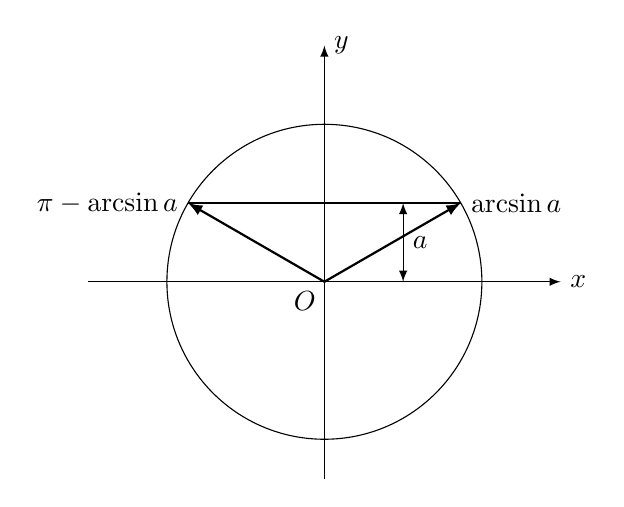
\begin{tikzpicture}[>=latex]
\draw[->] (-3,0)--(3,0)node[right]{$x$};
\draw[->] (0,-2.5)--(0,3)node[right]{$y$};
\node at (-.25,-.25){$O$};
\draw (0,0) circle(2);
\draw[thick,->] (0,0)--(30:2)node[right]{$\arcsin a$};
\draw[thick,->] (0,0)--(150:2)node[left]{$\pi-\arcsin a$};
\draw (30:2)--(150:2);
\draw[<->] (1,0)--node[right]{$a$}(1,1);

\end{tikzpicture}
    \caption{}
\end{figure}

    当$\arcsin a<x<\pi-\arcsin a$时,$f(x)=\sin x-a>0$成立;

    当$-\frac{\pi}{2}<x<\arcsin a$或$\pi-\arcsin a<x<\frac{3\pi}{2}$时,
    $f(x)=\sin x-a<0$成立,因此,在$|a|\le 1$的场合,$\sin x>a$
    在$\left[-\frac{\pi}{2}, \frac{3\pi}{2}\right]$内
    的解满足条件:
\[    \arcsin a<x<\pi-\arcsin a\]
由于$f(x)=\sin x-a$是周期等于$2\pi$的函数,因此
$\sin x>a$
的一切解满足条件:
\[2k\pi+\arcsin a<x<(2k+1)\pi-\arcsin a,\quad k\in\mathbb{Z}\]
\item  若$a>1$, 则对于任何$x\in\mathbb{R}$, 有$f(x)=\sin x-a<0$,因此,不等式$\sin x>a$没有解。
\item 若$a<-1$, 则对于任何$x\in\mathbb{R}$, 有$f(x)=\sin x-a>0$,
因此,不等式$\sin x>a$的解集是实数集$\mathbb{R}$。
\end{enumerate}

总之:
\begin{enumerate}
\item 当$|a|\le 1$时,所求不等式的解集是$$\{x|2k\pi+
\arcsin a<x<(2k+1)\pi-\arcsin a\}$$
\item 当$a>1$时,所求不等式的解集是空集$\emptyset$;
\item 当$a<-1$时,所求不等式的解集是实数集$\mathbb{R}$。
\end{enumerate}
\end{solution}


\begin{example}
    解不等式$\cos x<a$
\end{example}

\begin{solution}
移项,化为$\cos x-a<0$

设$f(x)=\cos x-a$, $f(x)$是周期等于$2\pi$的函数,先
讨论在长度等于一个周期的区间$[-\pi,\pi]$内的$f(x)$的符号:
\begin{enumerate}
    \item 若$|a|\le 1$, $f(x)=\cos x-a$在$[-\pi,\pi]$内的解是
\[x_1=\arccos a\quad \text{和}\quad x_2=-\arccos a\]
把解的终边画在单位圆上,如图9.20且由图9.20容易
看出:
\begin{figure}[htp]
    \centering
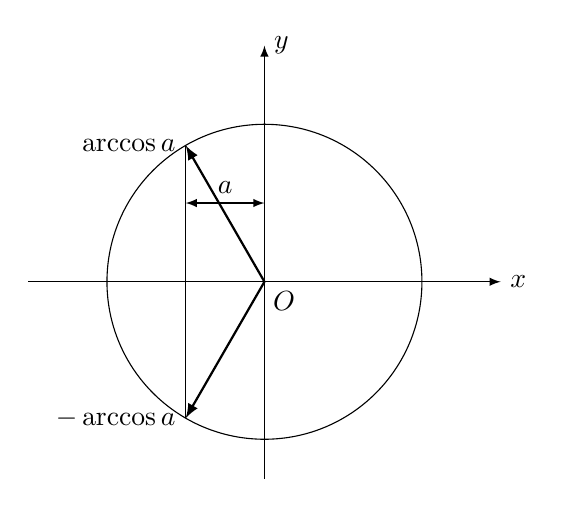
\begin{tikzpicture}[>=latex]
\draw[->] (-3,0)--(3,0)node[right]{$x$};
\draw[->] (0,-2.5)--(0,3)node[right]{$y$};
\node at (.25,-.25){$O$};
\draw (0,0) circle(2);
\draw[thick,->] (0,0)--(120:2)node[left]{$\arccos a$};
\draw[thick,->] (0,0)--(-120:2)node[left]{$-\arccos a$};
\draw (120:2)--(-120:2);
\draw[<->] (0,1)--node[above]{$a$}(-1,1);
\end{tikzpicture}
    \caption{}
\end{figure}

当$\arccos a<x<\pi$ 或$-\pi <x<-\arccos a$时,$f(x)=\cos x-
a<0$成立,而且仅在此时成立,又因为$f(x)=\cos x-a$的周期
是$2\pi$, 所以,$\cos x<a$的一切解,满足
\begin{equation}
   2k\pi +\arccos a<x<(2k+1)\pi  
\end{equation}
或
\begin{equation}
    (2k-1)\pi <x<2k\pi -\arccos a
\end{equation}
又(9.7)也可以写成
\begin{equation}
    (2k+1)\pi <x<(2k+2)\pi -\arccos a
\end{equation}
再将(9.6), (9.8)合并为
\begin{equation}
    2k\pi +\arccos a<x<(2k+2)\pi -\arccos a
\end{equation} 
因此,在$|a|\le 1$的场合,$\cos x<a$的一切解满足(9.9)。

\item 若$a>1$, 则对于任何$x\in\mathbb{R}$, 有
$f(x)=\cos x-a<0$成立,
因此,不等式$\cos x<a$的解集是实数集$\mathbb{R}$。
\item 若$a<-1$, 则对于任何$x\in\mathbb{R}$, 有
$f(x)=\cos x-a>0$成立,
因此,不等式$\cos x<a$没有解。
\end{enumerate}

总之,
\begin{enumerate}
\item 当$|a|\le 1$时,所求不等式的解集是
\[\{x|2k\pi  +\arccos a<x<(2k+2)\pi -\arccos a\}\]
\item 当$a>1$时,所求不等式的解集是实数集$\mathbb{R}$。
\item 当$a<-1$时,所求不等式的解集是空集$\emptyset$。
\end{enumerate}
\end{solution}


\begin{example}
    解不等式$2cos^2 2x<1$
\end{example}

\begin{solution}
移项,化简为$\cos4x<0$。设$f(x)=\cos4x$, 它是周期等于$\frac{2\pi}{4}=\frac{\pi}{2}$的函数。

$f(x)=\cos4x$在$\left[0,\frac{\pi}{2}\right]$内
的零点为$\frac{\pi}{8}$,$\frac{3\pi}{8}$。

显然,当$0\le x<\frac{\pi}{8}$时,$f(x)=\cos4x>0$;
当$\frac{\pi}{8}<x<\frac{3\pi}{8}$
时,$f(x)=\cos4x<0$;当$\frac{3\pi}{8}<x\le \frac{\pi}{2}$
时,$f(x)=\cos4x>0$。

$\therefore\quad \cos4x<0$在$\left[0,\frac{\pi}{2}\right]$内
的部分解满足条件:$\frac{\pi}{8}<x<\frac{3\pi}{8}$

又$f(x)$的周期是$\frac{\pi}{2}$。

$\therefore\quad \cos4x<0$的一切解满足条件
\[\frac{\pi}{8}+n\cdot\frac{\pi}{2}<x<\frac{3\pi}{8}+n\cdot\frac{\pi}{2}\qquad (n\in\mathbb{Z})\]
$\therefore\quad 2\cos^2 2x<1$的解集是
\[\left\{x\Big| \frac{\pi}{8}+n\cdot\frac{\pi}{2}<x<\frac{3\pi}{8}+n\cdot\frac{\pi}{2}\right\}\]
\end{solution}


\begin{example}
    解不等式$\frac{\cos2x+\cos x-1}{\cos2x}>2,\quad (0<x<2\pi)$
\end{example}

\begin{solution}
    移项,并将$\cos2x=2cos^2x-1$代入得
   \[\frac{\cos x(1-2\cos x)}{2cos^2x-1}>0\] 
    因为原不等式的解使$\cos2x\ne 0$(即$2cos^2x-1\ne 0$),两边乘
    以$(2\cos^x-1)^2$, 得到同解不等式
 \[   \cos x(1-2\cos x)(2\cos^2x-1)>0\]
    即
\[\left(\cos x+\frac{1}{\sqrt{2}}\right)\cos x\left(\cos x-\frac{1}{2}\right)\left(\cos x-\frac{1}{\sqrt{2}}\right)<0\]
上面不等式右端的函数式$f(x)$的零点依大小排列是
$-\frac{1}{\sqrt{2}},\; 0,\; \frac{1}{2},\; \frac{1}{\sqrt{2}}$。由此得知,仅当
\begin{equation}
    -\frac{1}{\sqrt{2}}<\cos x<0
\end{equation}
或
\begin{equation}
    \frac{1}{2}<\cos x<\frac{1}{\sqrt{2}}
\end{equation}
时,$f(x)=\cos x(1-2\cos x)(2\cos^2x-1)<0$。

由于$\cos x$在区间$[0,\pi]$内是递减的,在区间$[\pi,2\pi]$内
是递增的,所以由不等式(9.10), 得(图9.21):
\[\frac{\pi}{2}<x<\frac{3\pi}{4},\qquad \frac{5\pi}{4}<x<\frac{3\pi}{2}\]
由不等式(9.11), 得(图9.22):
\[\frac{\pi}{4}<x<\frac{\pi}{3},\qquad \frac{5\pi}{3}<x<\frac{7\pi}{4}\]
因此,原不等式在区间$0<x<2\pi$内的解集是
\[\left\{x\Big|\frac{\pi}{4}<x<\frac{\pi}{3} \right\}\bigcup\left\{x\Big|\frac{\pi}{2}<x<\frac{3\pi}{4} \right\}\bigcup\left\{x\Big|\frac{5\pi}{4}<x<\frac{3\pi}{2} \right\}\bigcup\left\{x\Big|\frac{5\pi}{3}<x<\frac{7\pi}{4} \right\}\]
\end{solution}

\begin{figure}[htp]\centering
    \begin{minipage}[t]{0.48\textwidth}
    \centering
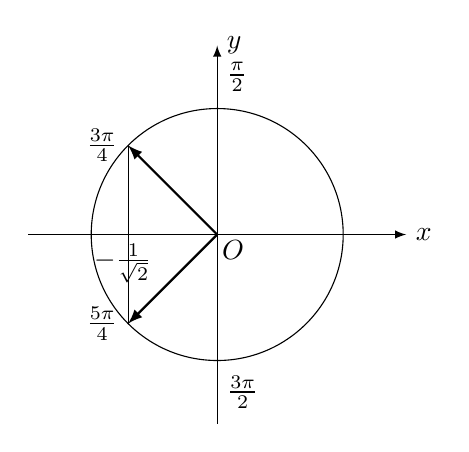
\begin{tikzpicture}[>=latex, scale=.8]
\draw[->] (-3,0)--(3,0)node[right]{$x$};
\draw[->] (0,-3)--(0,3)node[right]{$y$};
\node at (.25,-.25){$O$};
\draw (0,0) circle(2);
\draw[thick,->] (0,0)--(135:2)node[left]{$\frac{3\pi}{4}$};
\draw[thick,->] (0,0)--(-135:2)node[left]{$\frac{5\pi}{4}$};
\draw (135:2)--(-135:2);
\node at (0,2.5)[right]{$\frac{\pi}{2}$};
\node at (0,-2.5)[right]{$\frac{3\pi}{2}$};
\node at (-1.5,0)[below]{$-\frac{1}{\sqrt{2}}$};
    \end{tikzpicture}
    \caption{}
    \end{minipage}
    \begin{minipage}[t]{0.48\textwidth}
    \centering
    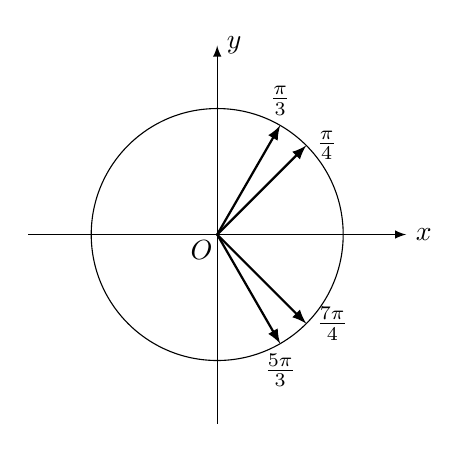
\begin{tikzpicture}[>=latex, scale=.8]
    \draw[->] (-3,0)--(3,0)node[right]{$x$};
\draw[->] (0,-3)--(0,3)node[right]{$y$};
\node at (-.25,-.25){$O$};
\draw (0,0) circle(2);
\draw[thick,->] (0,0)--(45:2)node[right]{$\frac{\pi}{4}$};
\draw[thick,->] (0,0)--(-45:2)node[right]{$\frac{7\pi}{4}$};
\draw[thick,->] (0,0)--(60:2)node[above]{$\frac{\pi}{3}$};
\draw[thick,->] (0,0)--(-60:2)node[below]{$\frac{5\pi}{3}$};


    \end{tikzpicture}
    \caption{}
    \end{minipage}
    \end{figure}



\section*{习题9.4}
\addcontentsline{toc}{subsection}{习题9.4}

\begin{enumerate}
    \item 解下列方程:
\begin{multicols}{2}
\begin{enumerate}
\item $\sin x=\frac{\sqrt{3}}{2}$
\item $\sin x=1$
\item $\sin\left(x+\frac{\pi}{6}\right)=-\frac{1}{2}$
\item $\sin x=0$
\item $\cos x=0$
\item $\cos\left(x+\frac{\pi}{6}\right)=\frac{1}{2}$
\item $\cos\left(x+\frac{\pi}{4}\right)=-\frac{\sqrt{3}}{2}$
\item $\cos x=1$
\item $\tan \left(x+\frac{\pi}{4}\right)=-1$
\item $\cot \frac{2x}{3}-1=0$
\item $\tan \left(x-\frac{\pi}{3}\right)=-\sqrt{3}$
\item $\cot x=0$
\end{enumerate}
\end{multicols}

    \item 解下列各方程(用反三角函数符号表示各方程的解):
\begin{multicols}{2}
\begin{enumerate}
\item $\sin2x=0.7$
\item $\cos\frac{\alpha}{2}=\frac{1}{5}$
\item $\tan 3x=3$
\item $\cot \frac{x}{4}=\frac{1}{4}$
    \item $\sin\left(\alpha+\frac{\pi}{3}\right)=0.1$
    \item $\cos\left(2x-\frac{\pi}{10}\right)=0.85$
    \item $\tan \left(\frac{x}{2}+\frac{\pi}{5}\right)=\frac{1}{8}$
    \item $\cot (2x-1)=\sqrt{2}$
\end{enumerate}
\end{multicols}

\item 解下列各方程:
\begin{enumerate}
    \begin{multicols}{2}
    \item $2 \sin \frac{x+1}{4}+1=0$
\item $4 \sin ^{2} 4 x-3=0$
\item $2 \sin ^{2} x-3 \sin x+1=0$
\item $\tan ^{2} 3 x=2 \tan  3 x$
 \end{multicols}
\item $\cot^{2}\left(\frac{x}{2}-\frac{\pi}{8}\right)+3 \cot\left(\frac{x}{2}-\frac{\pi}{8}\right)-4=0$
\item $4 \cos ^{2} x+\sin x=1$
\item $\tan  x+5 \cot x=6$
\item $2 \cot 3 x+\tan  3 x+3=0$
\end{enumerate}

\item $a,b,c$满足什么条件,方程$a\sin^2 x+b\cos^2 x=c$有解。

\item 解下列各方程:
   \begin{enumerate}
\item $\sin x(1+2 \cos x)=0$
\item  $\sin 2 x \cos 3 x=0$
\item  $\cos \left(2 x+\frac{\pi}{3}\right) \sin \left(3 x-\frac{\pi}{3}\right)=0$
\item  $\cos 5 x(1+\cos 2 x)=0$
\item $\cot x-\cos x=1-\sin x$
\item  $1+\sin x \cos 3 x+\sin x+\cos 3 x=0$
\item $\frac{\cos x}{1+\sin x}=2-\tan x$
\item $\sin 3 x \cdot \cot x=0$
\end{enumerate} 

\item 解下列各方程:
\begin{enumerate}
 \item  $\sin 3 x=\cos 3 x$
\item  $\sin ^{2} 3 x=3 \cos ^{2} 3 x$
\item $ 5 \cos x+2 \sin x=5 \cos x \cos 2 x+2 \sin x \cos 2 x$   
\item $\sin x \tan x+\cos x \cdot \cot x=\sin x+\cos x$
\item $\sin ^{2} x+5 \sin x \cos x+4 \cos ^{2} x=0$
\item $3 \sin ^{2} x-7 \sin x \cos x+6 \cos ^{2} x=1$
\item $\frac{\sin x+2 \cos x}{\sin x-2 \cos x}=3$
\item  $\frac{2 \sin ^{2} x-4 \cos ^{2} x}{\sin ^{2} x+3 \sin x \cos x+6 \cos ^{2} x}=1$
\end{enumerate}

\item $a, b$ 满足什么条件, 方程
$
\frac{a^{2} \sin x^{2}+b \cos x^{2}}{b^{2} \sin ^{2} x+a \cos x}=1
$有解。
\item 解下列各方程:
\begin{enumerate}
\item $\sin 3 x \cos x=\cos 3 x \sin x$
\item $\cos 7 x \cos 3 x=\cos 4 x$
\item $\sin \left(\frac{\pi}{2}-x\right) \cos 2 x+\sin (2 x-\pi) \sin x=0$
\item  $\sin \frac{3 \pi-x}{2} \cos \left(\frac{\pi}{2}-3 x\right) =\cos (3 x-\pi) \cos \frac{3 \pi+x}{2}$
\item $\tan x\cdot \tan\left(3x-\frac{\pi}{4}\right)=1$
\item $\sin x\cos x=\frac{1}{4}$
\item $\sin(34^{\circ}+x)\sin(56^{\circ}-x)=\frac{\sqrt{2}}{4}$
\item $\cos^4x-\sin^4x=1$
\item $\cos ^{2}\left(x+30^{\circ}\right)-\sin ^{2}\left(x+30^{\circ}\right)=\frac{1}{2}$
\item $\sin \left(x+\frac{\pi}{10}\right) \sin \left(\frac{2 \pi}{5}-x\right)=\frac{\sqrt{2}}{4}$
\begin{multicols}{2}
\item $\sin \left(x+\frac{\pi}{6}\right)=2 \cos x$
\item  $1-\tan^{2} x=2 \tan x \tan 2 x$
\item $2 \cos 2 x=7 \sin x $
\item  $\sin 2 x+\sqrt{2} \sin x=0$
\item  $2 \sin ^{2} x+\sin ^{2} 2 x=2$
\item  $\frac{\cos 2 x}{\cos x-\sin x}=0$
\item  $\sin 4 x=2 \cos ^{2} x-1 $
\item  $\sin x \cos x \cos 2 x=\frac{1}{8}$
\item  $\cot x-\tan x=\tan 2 x$
\item $2-\sin \frac{x}{2}=2 \cos \frac{x}{2}$
\end{multicols}
\end{enumerate}

\item 解下列各方程:

\begin{enumerate}
\item  $\sin 2 x=\sin 3 x$
\item  $\cos \left(2 x+15^{\circ}\right)=\cos \left(4 x-15^{\circ}\right)$
\item  $\tan\left(\frac{x}{2}+30^{\circ}\right)=\tan\left(2 x+60^{\circ}\right)$
\item  $\cos 3 x=\sin \left(x-\frac{\pi}{6}\right)$,
\item  $\tan\left(\frac{\pi}{8}-x\right)=\cot\left(\frac{\pi}{4}+3 x\right)$
\item  $\sin 2 x=-\sin \frac{x}{2}$
\item  $\tan 3 x+\cot \frac{x}{3}=0$
\item  $\sin 3 x+\frac{\sqrt{3}}{2} \sin 2 x=\frac{1}{2} \cos 2 x$
\item  $\cos x-\sin x=1$
\item  $\cos \left(2 x+15^{\circ}\right)+\cos \left(2 x-15^{\circ}\right)=\frac{1}{2}$
\item  $\sin x+\cos x=2 \sqrt{2} \sin x \cos x$
\item  $\sin 3 x \cos x=\sin 7 x \cos 5 x$
\item  $2 \cos \left(x+20^{\circ}\right) \cos x=\cos 40^{\circ} $
\item $\sin \left(2 x+\frac{\pi}{18}\right) \cos \left(2 x-\frac{\pi}{9}\right)=-\frac{1}{4}$
\item  $\sin \left(x+15^{\circ}\right) \sin \left(x-30^{\circ}\right)=$ $\sin \left(50^{\circ}+x\right) \cos \left(85^{\circ}-x\right)$
\end{enumerate}

\item 解下列各方程:
\begin{multicols}{2}
    \begin{enumerate}
\item $\cos 7 x+\cos x=\cos 4 x$
\item $\tan x+\tan 2 x=\sin 3 x \cos x$
\item $\cos 8 x+\cos 6 x=\sqrt{3} \cos x$
\item  $1-\cos 2 x=4 \sin x$
\item $\sin2 x+2\sin x=\sin\frac{x}{2}$
\item $\sin x+\sin 2x+ \sin 3x= 0$
\item $\cos x+\cos2x-\cos3x=1$
\item $\tan x+\tan 2x=\tan 3x$
\item $1+\cos2x+\sin x=2\cos^2\frac{x}{2}$

\end{enumerate}
\end{multicols}

\item 解下列各方程:
    \begin{enumerate}
\item $\sin ^{2}\left(x+10^{\circ}\right)-\sin ^{2} x=\frac{1}{2} \sin 20^{\circ}$
\item $\sin ^{2} x+\sin ^{2} 2 x+\sin ^{2} 3 x=\frac{3}{2}$
\item $\cos ^{2} x+\cos ^{2} 2 x+\cos ^{2} 3 x=1$
\item $\sin ^{2} 2 x+\sin ^{2} 4 x=\frac{3}{2}$
\item $\sqrt{3} \cos x+\sin x=\sqrt{3} $
\item $4 \sin x+3 \cos x=2 $
\item $\sin 3 x+2 \cos 2 x=1 $
\item  $5 \cos \left(2 x+18^{\circ}\right)-12 \sin \left(2 x+18^{\circ}\right)=13$
\item $(4 \sin x-5 \cos x)^{2}-13(4 \sin x-5 \cos x)+42=0$
\end{enumerate}


\item 解下列方程:
    \begin{enumerate}
\item $\frac{1+\tan x}{1-\tan x}=1+\sin 2 x$
\item $\frac{\sin x}{1+\cos x}=2-\cot x$
\item $\sin 2 x=\cos 2 x-\sin ^{2} x+1$
\item $(\cos 5 x+\cos 7 x)^{2}=(\sin 5 x+\sin 7 x)^{2}$
\end{enumerate}

\item 设关于$x$的方程$\sin x+\sqrt{3}\cos x+a=0$在区间内有
相异二解$\alpha,\beta$. 试求常数$a$的取值范围和$\tan(\alpha+\beta)$的值。
\item 解下列各方程组:
\begin{multicols}{2}
    \begin{enumerate}
\item $\begin{cases}
    \sin x\sin y=\frac{1}{4\sqrt{2}}\\
    \tan x\cdot \tan y=\frac{1}{3}
\end{cases}$
\item $\begin{cases}
    x+y=\frac{\pi}{4}\\
    \tan x+\tan y=1
\end{cases}$
\item $\begin{cases}
    \sin(2x+\sin^2y)=0\\
    x-3\sin^2y=-2
\end{cases}$
\end{enumerate}
\end{multicols}

\item 解下列的不等式:
\begin{enumerate}
\item $\sin (2 \pi \cos x)>0$
\item $\lg \sin x \leqslant 0$
\item $\cos ^{2} x+7 \sin ^{2} x<8 \sin x \cos x$
\item $2 \cos ^{2}\left(x+30^{\circ}\right)-3 \sin \left(60^{\circ}-x\right)+1>0$
\item $\sin x+\sqrt{3} \cos x>1$
\end{enumerate}


\item 求下列各函数的定义域:
\begin{multicols}{2}
   \begin{enumerate}
\item $y=\arccos \frac{3}{x}$
\item $y=\arcsin \frac{2 x}{1+x^{2}}$
\item $y=\sqrt{\sin x}$
\item $y=\sqrt{4 \cos ^{2} 2 x-3}$
\end{enumerate} 
\end{multicols}

\end{enumerate}




